% ============================================================
% Flight arrival delay prediction report
% Radhika Singhal
% Compile with pdfLaTeX (Overleaf default). Main file: report.tex
% Needs the 9 figure PDFs (fig1_workflow.pdf ... fig9_errors.pdf) in the folder figures/ next to this file.
% The appendix code is included below, so no other files are needed.
% ============================================================
\documentclass[12pt,a4paper]{article}
\usepackage[T1]{fontenc}
\usepackage[utf8]{inputenc}
\usepackage{mathptmx}
\usepackage[scaled=0.92]{helvet} % sans font for the cover page
\usepackage[margin=0.78in,top=0.75in,bottom=0.8in,columnsep=0.27in]{geometry}
\usepackage{microtype,graphicx,booktabs,array,multirow,caption,enumitem,listings,xcolor,amsmath,titlesec,fancyhdr,url}
\graphicspath{{figures/}}
\newcolumntype{R}[1]{>{\raggedright\arraybackslash}p{#1}}
\usepackage[colorlinks=true,linkcolor=black,citecolor=black,urlcolor=black]{hyperref}
\setlength{\emergencystretch}{2em}\setlength{\parindent}{1.1em}\setlength{\parskip}{0pt}\renewcommand{\baselinestretch}{1.03}
\titleformat{\section}{\normalsize\bfseries\scshape}{\thesection.}{0.5em}{}
\titleformat{\subsection}{\normalsize\bfseries\itshape}{\thesubsection}{0.5em}{}
\titlespacing*{\section}{0pt}{9pt}{3pt}\titlespacing*{\subsection}{0pt}{6pt}{2pt}
\definecolor{capgray}{gray}{0.40}
\captionsetup{font={footnotesize,sf,color=capgray},labelfont={bf,color=black},labelsep=period,skip=3pt}
\captionsetup[table]{position=top,skip=3pt}
% thin rules above and below every figure + caption, so the figure reads as one boxed unit apart from the body text.
% The bottom rule is added automatically; the top rule is written as \figrule on the line after each figure's \begin.
\usepackage{etoolbox}
\newcommand{\figrule}{\par\noindent{\color{black!50}\rule{\linewidth}{0.4pt}}\par}
\AtEndEnvironment{figure}{\figrule}
\AtEndEnvironment{figure*}{\figrule}
\brokenpenalty=10000 % never end a column on a hyphenated line (no "min-/utes" split across a figure)
\setlength{\textfloatsep}{12pt plus 2pt minus 4pt}
\setlist{nosep,leftmargin=1.2em}
\renewcommand{\arraystretch}{1.12}
\definecolor{hdrgray}{gray}{0.40}
\pagestyle{fancy}\fancyhf{}\fancyfoot[C]{\small\thepage}\renewcommand{\headrulewidth}{0pt}
\fancyhead[R]{\sffamily\footnotesize\color{hdrgray}Radhika Singhal}
\fancypagestyle{cover}{\fancyhf{}\fancyhead[R]{\sffamily\footnotesize\color{hdrgray}Radhika Singhal}\renewcommand{\headrulewidth}{0pt}}
\makeatletter
\renewcommand\tableofcontents{\section*{Contents}\begingroup\renewcommand{\baselinestretch}{0.97}\selectfont\renewcommand*\numberline[1]{##1\enspace}\@starttoc{toc}\endgroup}
\renewcommand*\l@section[2]{\vskip 0.5pt\noindent\textbf{#1}\nobreak\leaders\hbox{\,.\,}\hfill\nobreak\hbox to 1.4em{\hfill #2}\par}
\renewcommand*\l@subsection[2]{\noindent\hspace{1.2em}\small #1\nobreak\leaders\hbox{\,.\,}\hfill\nobreak\hbox to 1.4em{\hfill #2}\par}
\makeatother
\setcounter{tocdepth}{2}
\newcommand{\Fone}{$F_1$}
\newcommand{\code}[1]{\texttt{\small #1}}
\setcounter{topnumber}{3}\setcounter{totalnumber}{5}\renewcommand{\topfraction}{0.9}\renewcommand{\textfraction}{0.08}\renewcommand{\floatpagefraction}{0.75}
\lstdefinestyle{code}{language=Python,basicstyle=\ttfamily\fontsize{5.6}{6.45}\selectfont,breaklines=true,breakatwhitespace=false,keywordstyle=\bfseries,commentstyle=\itshape\color{black!60},stringstyle=\color{black!75},showstringspaces=false,columns=fullflexible,keepspaces=true,frame=none,aboveskip=2pt,belowskip=2pt,xleftmargin=0pt}

\begin{document}
% ------------------------------------------------------------ COVER PAGE
\thispagestyle{cover}
\begin{center}
\sffamily
\vspace*{0.26\textheight}
{\fontsize{32}{38}\selectfont\bfseries Flight Arrival Delay\\Prediction Report\par}
\vspace{16pt}
{\fontsize{15}{20}\selectfont\color{hdrgray} Introduction to Data Analytics, course project\par}
\vspace{40pt}
{\large Radhika Singhal\par}
\vspace{40pt}
{\large\color{hdrgray} October 2026\par}
\end{center}
\clearpage
\twocolumn
% ------------------------------------------------------------ ABSTRACT AND CONTENTS (two columns)
\section*{Abstract}
This report develops classifiers that predict whether a flight arrives delayed. Performance is measured by the \Fone{} score of the delayed class, the metric used by the Kaggle competition. Five required methods (Decision Tree, K-Nearest Neighbour, Random Forest, Support Vector Machine, Neural Network) and two extra models (Gradient Boosting, Logistic Regression) were tuned by cross-validation on 80\% of 42,634 labelled flights and evaluated on the remaining 20\%. Tuning for accuracy gave a Kaggle score of only 0.60, and tuning for \Fone{} raised it to 0.64. The decisive step was feature engineering: both files appear to be sorted by scheduled departure time, which makes it possible to estimate the unobserved departure delay and lifts every model by 14 to 18 points on the hold-out. Gradient Boosting performed best (cross-validated \Fone{} 0.853, hold-out 0.853, Kaggle 0.8471). The reliance on row order is a property of how the files were assembled and limits how far the result transfers to real deployments.

\tableofcontents
\vspace{4pt}
\section{Introduction}
\subsection{Problem and data}
Late arrivals disrupt passengers and airline operations, and identifying which flights arrive late supports rebooking, staffing and gate planning. The task is posed as binary classification: given the recorded attributes of a flight, predict \code{Arrival\_Delay} (1 = delayed, 0 = not delayed). The inputs are 15 attributes describing the origin, destination, airline, date, departure time, scheduled and elapsed duration, air time, distance, wheels-on time and taxi-in time. A labelled \emph{Flight} file of 42,634 flights is provided for model building, and an \emph{Unknown} file of 21,318 flights without labels is used for the final assessment through a Kaggle competition. Of the labelled flights, 32.8\% are delayed. A classifier that predicts ``not delayed'' for every flight is therefore 67.2\% accurate, but its \Fone{} for the delayed class is zero.

\subsection{Evaluation metric}
Kaggle ranks submissions by the \Fone{} score of the delayed class, $F_1 = 2PR/(P+R)$, where $P$ is precision and $R$ is recall among flights predicted delayed. \Fone{} ignores correctly predicted on-time flights, so it can differ sharply from accuracy when classes are imbalanced. This had a large practical effect. A first Decision Tree tuned for accuracy reached a Kaggle score of 0.6044, and tuning the same model for \Fone{} gave 0.6407 (Figure~\ref{fig:stages}). All later models were therefore tuned on \Fone{}, and the cut-off that turns a model score into a prediction was chosen to maximise \Fone{} (Section~\ref{sec:protocol}).

\subsection{Approach and workflow}
The work followed the steps in Figure~\ref{fig:workflow}. Missing values and routine derived features were handled inside a scikit-learn pipeline~\cite{sklearn}, so that every lookup table is learned from training rows only. The row-order and pooled estimates of the departure delay (Section~\ref{sec:hidden}) were computed beforehand from the supplied files, never using the labels, so the evaluation assumes each day's flight lists are available at prediction time. The labelled file was split into an 80\% training part and a 20\% hold-out part, and each classifier was tuned by randomised search with cross-validation on the training part alone. The cut-off was chosen on out-of-fold predictions, the hold-out gave the performance estimate, and the final model was refitted on all labelled flights before the Unknown file was scored. Kaggle scores served as a final check and not as an optimisation target (Section~\ref{sec:kaggle}).

\begin{figure*}[t]\figrule\vspace{1pt}
\centering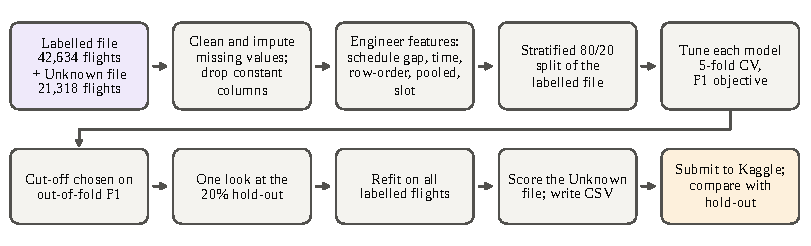
\includegraphics[width=0.92\textwidth]{fig1_workflow.pdf}
\caption{Workflow from the two raw files to the Kaggle submission. The hold-out part estimates final performance; it was also consulted in two exploratory comparisons (Section~\ref{sec:protocol}), so it is not a completely untouched test set.}\label{fig:workflow}
\end{figure*}

\subsection{Models used}
\textbf{Decision Tree}~\cite{cart} splits the data recursively on feature thresholds, giving readable rules; it over-fits unless depth and leaf size are limited. \textbf{K-Nearest Neighbour}~\cite{knn} labels a flight by the majority among its $k$ nearest training flights in standardised feature space; it needs no training but is sensitive to scale and to irrelevant features. \textbf{Random Forest}~\cite{rf} averages many trees grown on bootstrap samples with random feature subsets, which reduces variance. \textbf{Support Vector Machine}~\cite{svm} with an RBF kernel finds a maximum-margin boundary in a kernel-induced space, controlled by $C$ and $\gamma$. \textbf{Neural Network}~\cite{mlp} is a multilayer perceptron with ReLU hidden layers trained by back-propagation, with an L2 penalty and early stopping. Two extra models were added. \textbf{Gradient Boosting}~\cite{gb} adds small trees one at a time, each fitted to the errors of the ensemble so far. \textbf{Logistic Regression} is a linear baseline that shows how much non-linearity the problem contains.

\section{Dataset}
\subsection{Overview and exploratory analysis}
Both files cover 2015 and 334 distinct dates, with six airlines, 265 origin cities and 268 destination cities. October is absent from both files. The Unknown file has the same 15 attributes as the labelled file and no label. Departure and wheels-on times are stored as clock values (hhmm), and \code{SCHEDULED\_TIME} is the scheduled block duration in minutes. No scheduled departure time is supplied (Table~\ref{tab:attrs}).

\begin{table}[t]
\caption{Attributes of the Flight file (descriptions inferred from the values). The Unknown file has the same attributes except the target.}\label{tab:attrs}
\small\centering
\begin{tabular}{@{}l R{0.44\columnwidth}@{}}
\toprule
Attribute & Meaning\\
\midrule
\code{O\_CITY}, \code{O\_STATE} & origin city and state\\
\code{D\_CITY}, \code{D\_STATE} & destination city and state\\
\code{AIRLINE\_NAME}, \code{DATE} & operating airline; flight date\\
\code{DEPARTURE\_TIME} & actual departure time (hhmm)\\
\code{SCHEDULED\_TIME} & scheduled duration (minutes)\\
\code{ELAPSED\_TIME}, \code{AIR\_TIME} & actual and airborne duration (minutes)\\
\code{DISTANCE} & route distance\\
\code{WHEELS\_ON}, \code{TAXI\_IN} & landing time (hhmm); taxi time to the gate\\
\code{DIVERTED}, \code{CANCELLED} & event flags\\
\code{Arrival\_Delay} & \textbf{target}: 1 = delayed, 0 = not delayed\\
\bottomrule
\end{tabular}
\end{table}

Figure~\ref{fig:eda} shows the main patterns. The delayed share rises steadily through the day, from 12\% for 05:00 departures to 51\% for 22:00 departures, which is consistent with delays accumulating as the day progresses. Airlines differ only modestly (27\% for Delta Air Lines to 36\% for SkyWest). The strongest single signal is the schedule gap, $\mathrm{DIFF} = \mathrm{ELAPSED\_TIME} - \mathrm{SCHEDULED\_TIME}$, whose area under the ROC curve (AUC) is 0.736 on its own. The significance of these patterns differs. Time of day separates flights well (a 39-point spread, against 9 points between airlines), so departure time enters the models in several forms while the airline is a minor input. The schedule gap matters for a more direct reason: it is the time a flight spent beyond its schedule, one of the two quantities whose sum the label closely follows (Section~\ref{sec:hidden}), and it is also recorded in the Unknown file.

\begin{figure*}[t]\figrule\vspace{1pt}
\centering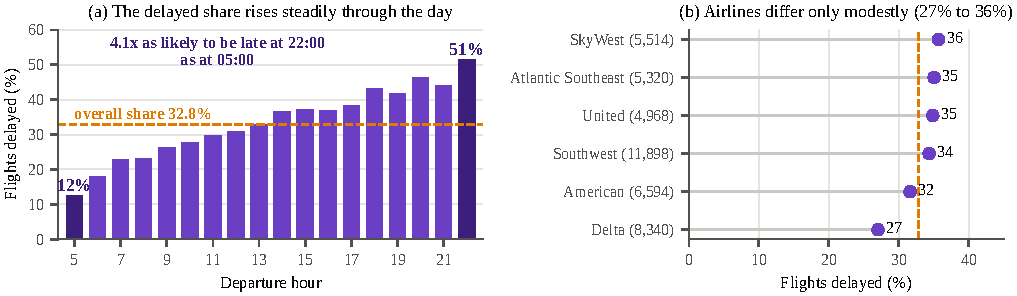
\includegraphics[width=0.92\textwidth]{fig2_eda.pdf}
\caption{Delayed share by departure hour (a) and by airline (b); the dashed line is the overall share of 32.8\%. Time of day is the strongest pattern: the share rises from 12\% for 05:00 departures to 51\% for 22:00 departures, about four times as high, whereas the six airlines span only 27\% to 36\%. Hours with fewer than 1,000 flights are omitted; airline flight counts are in brackets.}\label{fig:eda}
\end{figure*}

\subsection{Missing values and preprocessing}
\begin{figure}[t]\figrule\vspace{1pt}
\centering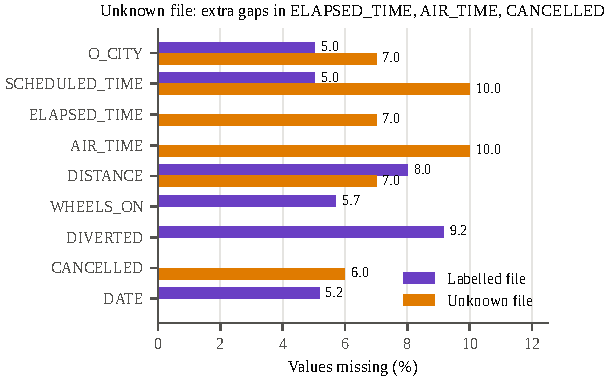
\includegraphics[width=\columnwidth]{fig3_missing.pdf}
\caption{Share of values missing in each file. The Unknown file has extra gaps (6\% to 10\%, at round rates) in \code{ELAPSED\_TIME} and \code{AIR\_TIME}, which are complete in the labelled file, and in \code{CANCELLED}, a constant flag that is dropped. The duration features must therefore be imputed at prediction time.}\label{fig:missing}
\end{figure}
Figure~\ref{fig:missing} shows that missingness differs between the files. Both files have gaps in three columns (\code{O\_CITY}, \code{SCHEDULED\_TIME} and \code{DISTANCE}). The labelled file also has gaps in \code{WHEELS\_ON}, \code{DIVERTED} and \code{DATE}. The Unknown file additionally has gaps in \code{ELAPSED\_TIME}, \code{AIR\_TIME} and \code{CANCELLED}, which are complete in the labelled file. The Unknown rates are round numbers (6\%, 7\% and 10\%), which suggests the gaps were inserted at random. The pipeline therefore had to impute the duration columns at prediction time, although they were complete in training; \code{CANCELLED} is dropped (below). The following rules were applied.
\begin{itemize}
\item \textbf{Cancelled and diverted flights.} \code{CANCELLED} is 0 and \code{DIVERTED} is 0 wherever they are recorded, so neither file contains a cancelled or diverted flight. Both columns are constant and carry no information, so they were dropped. A consequence is that the models are not validated for such flights and should not be applied to them.
\item \textbf{Date.} 5.2\% of labelled dates are missing. Because the file is sorted by date (checked in code before use), each gap was filled from the nearest earlier known date.
\item \textbf{Durations, distance and wheels-on time.} Gaps were filled with the median of the same city route, then of the same state route, followed by regressions on related columns. For example, elapsed time follows from departure and wheels-on times, and air time was regressed on related durations. Distance is constant per route.
\item \textbf{Origin city.} Missing values became an explicit \code{UNK} category, because the origin state is always present.
\item \textbf{Geography.} City and state were used for imputation only. Target-encoding of routes and cities was tested in an ablation and gave no measurable gain, and KNN scored slightly lower with it, so geography is not offered to the models directly.
\end{itemize}
Derived features include the schedule gap and its ratio, clock features of departure and arrival (hour, sine and cosine, a pre-dawn flag), taxi-out time, speed, calendar fields, a one-hot airline encoding and an out-of-fold target encoding of the date (334 values are too many for one-hot encoding). Scaling was applied only for KNN, SVM, the Neural Network and Logistic Regression.

\begin{figure}[t]\figrule\vspace{1pt}
\centering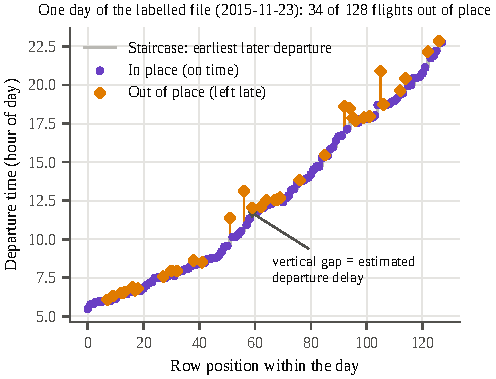
\includegraphics[width=\columnwidth]{fig4_order.pdf}
\caption{Departure time against row position for one day (34 of its 128 flights are out of place). Flights that left on time (blue) follow a rising staircase; flights that left late (orange) sit above it, and the vertical gap to the staircase estimates their departure delay. The row order of the file therefore carries information about delay.}\label{fig:order}
\end{figure}
\subsection{Hidden structure in the data}\label{sec:hidden}
A closer inspection of the files revealed regularities that are not described in the assignment brief and that strongly affect modelling (Table~\ref{tab:hidden}).

\begin{table*}[t]
\caption{Hidden structure found in the two files and its consequence for modelling.}\label{tab:hidden}
\small\centering
\begin{tabular}{@{}c R{0.17\textwidth} R{0.40\textwidth} R{0.31\textwidth}@{}}
\toprule
\# & Finding & Evidence & Consequence\\
\midrule
1 & Rows are sorted by date, then by scheduled departure time & Within a day, the correlation of row position with departure clock time averages 0.97 over 334 days (Unknown file: 0.97). Late flights sit out of place (Figure~\ref{fig:order}). & Departure delay can be estimated from row order (\code{DEP\_DELAY\_EST}).\\
2 & The two files differ in density & The median day has 128 flights in the labelled file and 64 in the Unknown file. & Features are computed in labelled halves of about 64 flights per day, matching the Unknown file.\\
3 & Some flights recur & 19\% of flights have at least two other copies (same airline, route and block time) within $\pm$45 days across the three lists. & Pooling copies gives a sharper schedule estimate (pooled features).\\
4 & The label turns on at about 5 minutes late & Among flights that left in place, the delayed share by schedule gap (min) is 1.5\% ($\le 0$), 4.5\% (0--2), 20\% (2--5), 54\% (5--8), 89\% (8--10) and 100\% ($>$10); $n = 420$, small above 5 minutes. & The label is close to ``arrived more than a few minutes behind schedule'', not the common 15-minute rule.\\
5 & Missingness differs by file & Round rates (6\%, 7\%, 10\%) in the Unknown file; different columns affected (Figure~\ref{fig:missing}). & Imputation must cover columns complete in training.\\
6 & Constant columns; identical dates & \code{CANCELLED} and \code{DIVERTED} are always 0. Both files cover the same 334 dates, and October is absent from both. & Constants dropped; day-level information learned from the labelled file transfers to the Unknown file; no generalisation to October.\\
\bottomrule
\end{tabular}
\end{table*}

\paragraph{Departure delay from row order.} A flight that left on time appears at the position its departure time implies. A flight that left late appears out of place, with a departure time later than flights listed after it (Figure~\ref{fig:order}). Its scheduled departure can therefore be bounded by the earliest actual departure among the flights listed after it that day (the suffix minimum), and the difference estimates the departure delay. This quantity matters because an arrival delay is largely the departure delay plus any extra time on the route. Alone, the schedule gap and the estimated departure delay reach AUC values of 0.736 and 0.731, but their sum reaches 0.903. These features use only departure times and row order, never the label, and are computed identically for the Unknown file. They also describe a property of how the files were assembled and not a property of flights, a limitation returned to in Section~\ref{sec:conclusion}.


\paragraph{Why the two signals matter.} Figure~\ref{fig:signals} shows why the schedule gap and the estimated departure delay are the most relevant quantities in the data. Among flights estimated to have left on time, the delayed share rises from 8\% when the schedule gap is zero or negative to 62\% at 5 to 8 minutes of extra time and above 94\% beyond 10 minutes, and flights whose neighbours in the file left within 4 minutes show the same step more sharply (Table~\ref{tab:hidden}, row 4). The label therefore switches on after a few minutes of extra time, not at the 15-minute threshold of official on-time statistics. The estimated departure delay behaves in the same way: the delayed share climbs from 20\% to 99\% as the estimate grows from zero to 30 to 60 minutes. The slightly lower share above 60 minutes (92\%) is probably noise in very large estimates and was not investigated. The significance of the pair is that the signals are complementary: each alone has an AUC of about 0.73, yet together they reach 0.903, because a flight arrives late when its departure delay and its extra time on the route add up to more than a small margin. Their relevance is practical, since neither is a column in the files; one is derived from elapsed and scheduled time and the other is recovered from the row order.

\begin{figure*}[t]\figrule\vspace{1pt}
\centering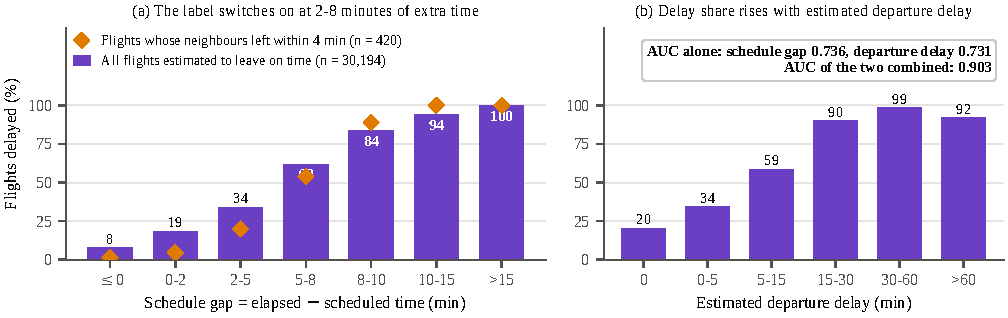
\includegraphics[width=0.92\textwidth]{fig8_signals.pdf}
\caption{Why the two engineered signals matter. (a) Among flights estimated to leave on time, the delayed share jumps from 8\% to 62\% as the schedule gap grows from at most zero to 5 to 8 minutes, and exceeds 94\% beyond 10 minutes; flights whose neighbours left within 4 minutes (orange) show the same step more sharply. (b) The delayed share rises from 20\% to 99\% as the estimated departure delay grows to 30 to 60 minutes. Each signal alone has an AUC of about 0.73; together they reach 0.903.}\label{fig:signals}
\end{figure*}

\paragraph{Matching the Unknown file.} The Unknown file holds 64 flights per day and the labelled file 128, so order-based estimates computed on the full labelled file would be sharper than any estimate available at prediction time. A model trained on such features would meet noisier features on the Unknown file. The labelled file was therefore split at random into two halves of about 64 flights per day, and the features were computed within each half, which gives training and Unknown features the same density. Merging the two files into one list to recover the full day was tried in five variants and scored lower each time, because their interleaving cannot be recovered exactly.

\paragraph{Pooled and slot features.} Where the same flight recurs on nearby days, each copy yields its own bound, and the tightest consistent bound over $\pm$45 days (pooled across both labelled halves and the Unknown file) gives a better estimate of the scheduled departure; this adds six pooled features. Twelve slot features encode the departure minute within 5-, 10-, 15-, 30- and 60-minute blocks and the candidate delays if the flight had been early or late relative to a nearby 5-minute mark. The assumption that schedules sit on 5-minute marks is not visible in the raw departure minutes (21\% fall on multiples of five, against 20\% expected by chance), and this group raised the Gradient Boosting hold-out \Fone{} by only 0.5 points, within sampling error. It was retained, but its benefit is regarded as unproven.

\section{Models and Tuning}
\subsection{Validation protocol}\label{sec:protocol}
The labelled file was split once into a stratified 80\% training part (34,107 flights) and a 20\% hold-out part (8,527 flights), with a fixed random seed. All tuning used the training part only. Each model was tuned by randomised search over the grids in Table~\ref{tab:params}, scored by cross-validated \Fone{} maximised over cut-offs. For every model except the Decision Tree these cut-offs flag between 15\% and 60\% of flights; the Decision Tree searched fixed probability thresholds from 0.10 to 0.80. The chosen model produced out-of-fold predictions (every flight scored by a model that never saw it), and the final cut-off was the median of the cut-offs whose out-of-fold \Fone{} lay within 0.001 of the maximum (for the Decision Tree, on a fixed probability grid from 0.10 to 0.80), which avoids selecting a single noisy peak. The hold-out was then evaluated for each final model (its use in exploratory comparisons is described under Leakage controls), and the final model was refitted on all labelled flights. Three estimates are reported for every model: in-sample, cross-validated and hold-out \Fone{}. For KNN, Random Forest and SVM, the in-sample value is uninformative because these models can fit their training flights almost perfectly.

\paragraph{Leakage controls.} Imputation tables, scalers and encoders are fitted inside the pipeline on the training rows of each fold only, and the date encoding is computed out-of-fold. The row-order and pooled features use departure times and positions, never labels, but are built from the labelled and Unknown files before the split, so the evaluation assumes each day's flight lists are available at prediction time (Section~\ref{sec:conclusion}). Because both files cover the same 334 dates, a random split mirrors the relation between the labelled and Unknown files, so day-level information learned from training flights is legitimately available at prediction time. The hold-out was not used to tune hyperparameters or choose the cut-off, but it was used in two exploratory comparisons: whether to keep the slot group for each model (Section~\ref{sec:ladder}) and the wider-search check in Section~\ref{sec:robust}, which did not change the model. The differences were within noise, but the hold-out is not a completely untouched test set.

\begin{table*}[t]
\caption{Search settings and chosen parameters. Search = number of random settings $\times$ cross-validation folds. ``compact+date'' = raw columns, schedule gap and row-order features, standardised, plus the out-of-fold date encoding.}\label{tab:params}
\footnotesize\centering
\begin{tabular}{@{}l R{0.07\textwidth} R{0.38\textwidth} R{0.315\textwidth}@{}}
\toprule
Model & Search & Search space & Chosen parameters\\
\midrule
Decision Tree & $60\times5$ & max\_depth \{4--20, none\}; min\_samples\_leaf \{10--200\}; criterion \{gini, entropy\}; ccp\_alpha \{0--$10^{-3}$\}; class\_weight \{none, balanced, 1:1.5\}; max\_leaf\_nodes \{none, 30--250\}; min\_impurity\_decrease \{0, $10^{-4}$, $5\!\times\!10^{-4}$\} & max\_depth 8; min\_samples\_leaf 10; max\_leaf\_nodes 60; gini; ccp\_alpha $2\!\times\!10^{-4}$; no class weights\\
KNN & $20\times3$ & $k$ \{5, 11, 21, 31, 51, 75, 101\}; weights \{uniform, distance\}; Minkowski $p$ \{1, 2\}; feature set \{full, compact, compact+date\} & $k=75$; distance weights; $p=1$ (Manhattan); compact+date\\
Random Forest & $15\times3$ & n\_estimators \{200, 400\}; max\_depth \{8, 12, 16, none\}; min\_samples\_leaf \{1, 3, 5, 10, 20\}; max\_features \{sqrt, 0.3, 0.5\}; class\_weight \{none, balanced\_subsample\} & 400 trees; no depth limit; min\_samples\_leaf 3; max\_features sqrt; no class weights\\
SVM (RBF) & $12\times3$ on 8,000 rows & $C$ \{0.5, 1, 2, 5, 10\}; $\gamma$ \{scale, 0.01, 0.03, 0.1\}; class\_weight \{none, balanced\}; feature set \{full, compact, compact+date\} & $C=1$; $\gamma=0.03$; balanced weights; compact+date; refitted on all training rows\\
Neural Network & $10\times3$ & hidden layers \{(32), (64), (64,32), (128,64)\}; L2 $\alpha$ \{$10^{-5}$--$10^{-2}$\}; initial learning rate \{0.001, 0.003\}; early stopping (patience 10, max 300 epochs) & layers (64, 32); $\alpha=10^{-4}$; learning rate 0.001\\
Gradient Boosting & $15\times5$ & learning\_rate \{0.02, 0.03, 0.05, 0.1\}; max\_leaf\_nodes \{15, 31, 63\}; min\_samples\_leaf \{20, 30, 50, 100\}; l2 \{0, 1, 10\}; class\_weight \{none, balanced\}; early stopping (10\% validation, patience 50, max 3,000 iterations) & learning rate 0.05; 31 leaves; min\_samples\_leaf 30; l2 1; no class weights\\
Logistic Regression & $12\times5$ & $C$ \{0.01, 0.03, 0.1, 1, 10, 100\}; class\_weight \{none, balanced\}; feature set \{full, compact+date\} & $C=0.1$; balanced weights; compact+date\\
\bottomrule
\end{tabular}
\end{table*}

\subsection{Model notes}
\textbf{Decision Tree.} A larger search (60 settings, five folds) was used because single trees are unstable. Depth, leaf size and cost-complexity pruning limit memorisation; the chosen tree has at most 60 leaves. Its in-sample and cross-validated \Fone{} (0.849 and 0.833) are close, which indicates little over-fitting. A tree of depth three already reaches a hold-out accuracy of 0.890, and its first split is on the candidate arrival delay at a threshold of about 7 minutes, which shows how simple the underlying rule is once the key features exist.

\textbf{KNN.} Distance-based methods suffer when many features are irrelevant, so the search could choose a compact feature set, and the chosen set contains only the raw columns, the schedule gap, the row-order features and the date encoding. A large $k$ of 75 with distance weighting and Manhattan distance gave the best cross-validated \Fone{}.

\textbf{Random Forest.} Averaging 400 deep trees with random feature subsets (square-root rule) gave a strong, stable model. The gap between in-sample \Fone{} (0.961) and cross-validated \Fone{} (0.845) is expected for a forest and is not itself evidence of over-fitting.

\textbf{SVM.} Training time grows roughly with the square of the number of rows, so the search ran on a stratified subsample of 8,000 training flights and the chosen settings were refitted on all training rows. Balanced class weights and a moderate $C$ were preferred.

\textbf{Neural Network.} A small network of two hidden layers was chosen over wider ones. Early stopping on an internal validation slice and the L2 penalty control over-fitting.

\textbf{Logistic Regression.} The linear baseline reaches a hold-out \Fone{} of 0.789, 6 points below the next model, so the interaction between schedule gap and departure delay is clearly non-linear.

\section{Results and Comparison}
\subsection{Estimated test error}
Table~\ref{tab:results} reports the three \Fone{} estimates and the hold-out precision, recall and AUC, together with cross-validated \Fone{} under two other splits (90/10 and 100/0, the latter with no hold-out). Figure~\ref{fig:models} compares the reported performance estimates with the Kaggle scores. Tuning cost differed widely on a two-core machine: 19 s for Logistic Regression, 31 s for the Neural Network, 43 s for the SVM (on its subsample), 118 s for KNN, 127 s for the Decision Tree, 222 s for Gradient Boosting and 782 s for Random Forest.

\begin{table*}[t]
\caption{Results by model: \Fone{} of the delayed class (in-sample, 5-fold or 3-fold cross-validated, hold-out), hold-out precision, recall and AUC, and cross-validated \Fone{} under 90/10 and 100/0 splits. In-sample values for KNN, Random Forest and SVM are not informative.}\label{tab:results}
\small\centering
\begin{tabular}{@{}l ccc ccc cc@{}}
\toprule
 & \multicolumn{3}{c}{\Fone{} (80/20 split)} & \multicolumn{3}{c}{Hold-out (80/20)} & \multicolumn{2}{c}{CV \Fone{}}\\
\cmidrule(lr){2-4}\cmidrule(lr){5-7}\cmidrule(lr){8-9}
Model & In-sample & CV & Hold-out & Precision & Recall & AUC & 90/10 & 100/0\\
\midrule
Gradient Boosting & 0.904 & 0.853 & \textbf{0.853} & 0.860 & 0.847 & 0.962 & 0.853 & 0.854\\
Random Forest & 0.961 & 0.845 & 0.848 & 0.874 & 0.824 & 0.957 & 0.845 & 0.846\\
Neural Network & 0.864 & 0.842 & 0.839 & 0.863 & 0.817 & 0.956 & 0.841 & 0.842\\
SVM (RBF) & 0.858 & 0.840 & 0.837 & 0.849 & 0.826 & 0.954 & 0.838 & 0.837\\
Decision Tree & 0.849 & 0.833 & 0.833 & 0.858 & 0.810 & 0.940 & 0.833 & 0.835\\
KNN & 0.991 & 0.825 & 0.825 & 0.824 & 0.825 & 0.946 & 0.824 & 0.825\\
Logistic Regression & 0.788 & 0.783 & 0.789 & 0.787 & 0.791 & 0.917 & 0.784 & 0.783\\
\bottomrule
\end{tabular}
\end{table*}

\begin{figure*}[t]\figrule\vspace{1pt}
\centering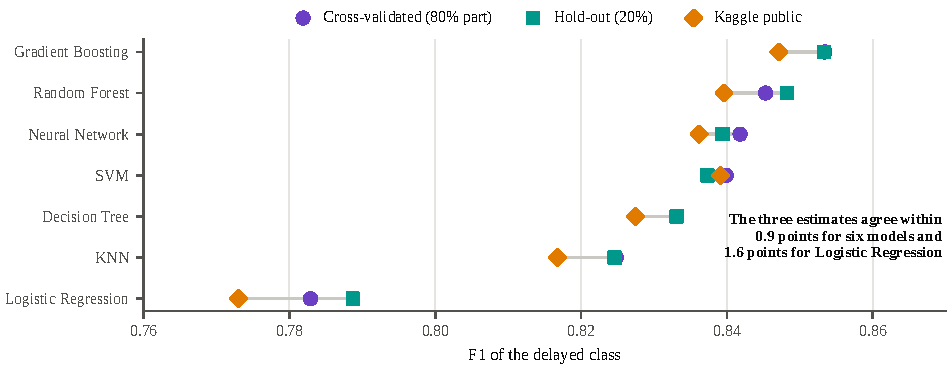
\includegraphics[width=0.86\textwidth]{fig6_models.pdf}
\caption{Cross-validated, hold-out and Kaggle \Fone{} by model. The three estimates agree within 0.9 points for six models and within 1.6 points for Logistic Regression, and Gradient Boosting is highest on all three.}\label{fig:models}
\end{figure*}

\subsection{Kaggle submissions}
Table~\ref{tab:kaggle} lists the Kaggle public scores of all seven models. Every model improved as the feature set was refined, and Figure~\ref{fig:stages} shows the development path: tuning for \Fone{} added 3.6 points, and the row-order features added a further 17 to 19 points on Kaggle (Decision Tree: 0.6407 to 0.8080; Gradient Boosting v2: 0.8308, from the same starting point). Logistic Regression, the extra baseline, scored 0.7730.

\begin{table}[t]
\caption{Kaggle public \Fone{} of every model. The final version is the one used in this report.}\label{tab:kaggle}
\small\centering
\begin{tabular}{@{}l p{0.38\columnwidth} c@{}}
\toprule
Model & Earlier versions & Final\\
\midrule
Gradient Boosting & v2: 0.8308 & \textbf{0.8471}\\
Random Forest & none & 0.8396\\
SVM (RBF) & v2: 0.8238 & 0.8391\\
Neural Network & v2: 0.8254 & 0.8362\\
Decision Tree & attempt 1: 0.6044; 2: 0.6407; 4: 0.8080 & 0.8275\\
KNN & v2: 0.8068 & 0.8168\\
Logistic Regression & none & 0.7730\\
\bottomrule
\end{tabular}
\end{table}

\begin{figure}[t]\figrule\vspace{1pt}
\centering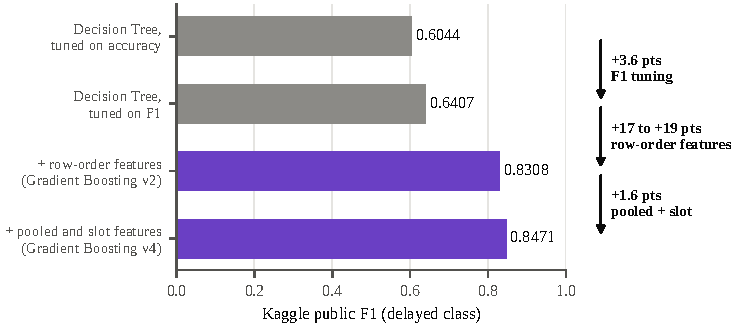
\includegraphics[width=\columnwidth]{fig5_stages.pdf}
\caption{Kaggle public \Fone{} at four stages of development. Tuning for \Fone{} instead of accuracy added 3.6 points, the row-order features added a further 17 to 19 points, and the pooled and slot features added 1.6 points. Grey bars: Decision Tree before the row-order features; blue bars: Gradient Boosting after them.}\label{fig:stages}
\end{figure}

\subsection{Effect of the feature groups}\label{sec:ladder}
Table~\ref{tab:ladder} repeats the evaluation as the feature groups were added. The row-order group raised the six non-linear models by 16 to 18 points and Logistic Regression by 14; the pooled group added 1 to 2 points; the slot group helped only Gradient Boosting (0.5 points), KNN and the Decision Tree (0.1 to 0.2 points), left Random Forest and the SVM unchanged and slightly lowered the Neural Network and Logistic Regression. The slot group was therefore used only for Gradient Boosting, KNN and the Decision Tree, and the other four final models use the pooled feature set.

\begin{table}[t]
\caption{Hold-out \Fone{} (80/20 split) as feature groups were added. Final models: Gradient Boosting, Decision Tree and KNN with all groups; the others with the pooled set.}\label{tab:ladder}
\small\centering\setlength{\tabcolsep}{3.5pt}
\begin{tabular}{@{}l cccc@{}}
\toprule
Model & Base & +Order & +Pooled & +Slot\\
\midrule
Gradient Boosting & 0.660 & 0.838 & 0.848 & \textbf{0.853}\\
Random Forest & 0.661 & 0.834 & \textbf{0.848} & 0.848\\
Neural Network & 0.657 & 0.821 & \textbf{0.839} & 0.838\\
SVM (RBF) & 0.653 & 0.823 & \textbf{0.837} & 0.837\\
Decision Tree & 0.640 & 0.816 & 0.832 & \textbf{0.833}\\
KNN & 0.645 & 0.811 & 0.823 & \textbf{0.825}\\
Logistic Reg. & 0.634 & 0.770 & \textbf{0.789} & 0.787\\
\bottomrule
\end{tabular}
\end{table}

\subsection{Quantitative analysis}\label{sec:kaggle}
\textbf{Model ranking.} The ranking is consistent across the three reported performance estimates: Gradient Boosting leads, followed by Random Forest, then the Neural Network and SVM, then the Decision Tree and KNN, with Logistic Regression last. On Kaggle the order of the middle group changes slightly (SVM 0.8391 against Neural Network 0.8362), but the differences between neighbouring models are 0.3 to 0.8 points, within sampling error. Logistic Regression is last on Kaggle too (0.7730). The lead of Gradient Boosting over Random Forest (0.5 points) is likewise small, whereas its lead of 1.4 to 2.8 points over the SVM, Neural Network, Decision Tree and KNN is more reliable.

\textbf{Reliability of the estimates.} The assignment cautions that the public Kaggle score covers only part of the test data and must not be used as the test error or optimised against. Models were therefore selected on cross-validated and hold-out \Fone{}, and Kaggle scores were consulted only afterwards. Hold-out and Kaggle agree within one point for six of the seven models (differences from $-0.9$ to $+0.2$ points), as expected from sampling error alone, since a hold-out of 8,527 flights has a standard error of roughly 0.7 points. Logistic Regression is the exception ($-1.6$ points), possibly because a linear model copes less well with the Unknown file's extra missing values (not tested). The differences are mostly negative, which is consistent with mild optimism from choosing settings and cut-offs on the training part and possibly with the extra missingness in the Unknown file. The hidden private score will differ somewhat; all figures here are estimates.

\textbf{Splits and over-fitting.} Cross-validated \Fone{} changes by at most 0.3 points between the 80/20, 90/10 and 100/0 splits (Table~\ref{tab:results}), so the conclusions do not depend on the split. Cross-validated and hold-out \Fone{} agree within 0.6 points for every model.

\section{Best Model: Gradient Boosting}
\subsection{Choice and architecture}
Gradient Boosting was selected because it has the highest cross-validated \Fone{} (0.853), the highest hold-out \Fone{} (0.853) and the highest Kaggle score (0.8471), and it is the most consistent of the models across splits. The implementation is scikit-learn's histogram-based \code{HistGradientBoostingClassifier}. Trees are added sequentially, each fitted to the gradient of the log-loss of the current ensemble and shrunk by the learning rate~\cite{gb}; features are binned, no scaling is needed, and training stops early when an internal 10\% validation slice stops improving. The chosen model uses a learning rate of 0.05, trees of at most 31 leaves, at least 30 flights per leaf and an L2 penalty of 1 (Table~\ref{tab:params}). It receives 54 input columns grouped as in Table~\ref{tab:features}.

\begin{table}[t]
\caption{Feature groups of the final Gradient Boosting model (54 input columns).}\label{tab:features}
\small\centering
\begin{tabular}{@{}l c p{0.58\columnwidth}@{}}
\toprule
Group & $n$ & Examples\\
\midrule
Base & 28 & schedule gap, clock and calendar fields, taxi-out, speed, airline, date encoding\\
Row order & 8 & \code{DEP\_DELAY\_EST}, neighbour gaps, estimated total delay\\
Pooled & 6 & \code{PDELAY}, support counts, window width\\
Slot & 12 & minute-block offsets, candidate delays\\
\bottomrule
\end{tabular}
\end{table}

\subsection{How it solves the problem}
The label is close to a threshold on the sum of two quantities: the extra time spent on the route (the schedule gap) and the departure delay. The first is observed; the second is estimated from the row order. Gradient Boosting can model the interaction of these quantities, and of their sum, with the time of day and the airline, without the scaling that distance-based models need. Table~\ref{tab:ladder} shows that nearly all of its accuracy comes from the engineered features: the base columns give a hold-out \Fone{} of 0.660, the row-order group lifts it to 0.838, and the pooled and slot groups add 1.0 and 0.5 points.

\paragraph{Which inputs matter.} Figure~\ref{fig:errors} (a) shuffles each group of input columns in the hold-out set and records the fall in \Fone{} (five repetitions; the bars show one standard deviation). Shuffling the 12 columns that carry the row-order and pooled information lowers \Fone{} by 0.302, and shuffling the schedule gap and duration columns lowers it by 0.264, whereas departure time (0.016), geography (0.017), date (0.011) and airline (0.004) matter little. The model therefore rests almost entirely on the two signals of Section~\ref{sec:hidden}. Airline is the least important group, in line with the small differences between airlines in Figure~\ref{fig:eda}. The geography columns are used only to fill gaps, so their small effect reflects less accurate imputation and not a direct use. Group importance is a rough guide, because groups that carry related information, such as departure time and the row-order features, can share credit unevenly.

\begin{figure*}[t]\figrule\vspace{1pt}
\centering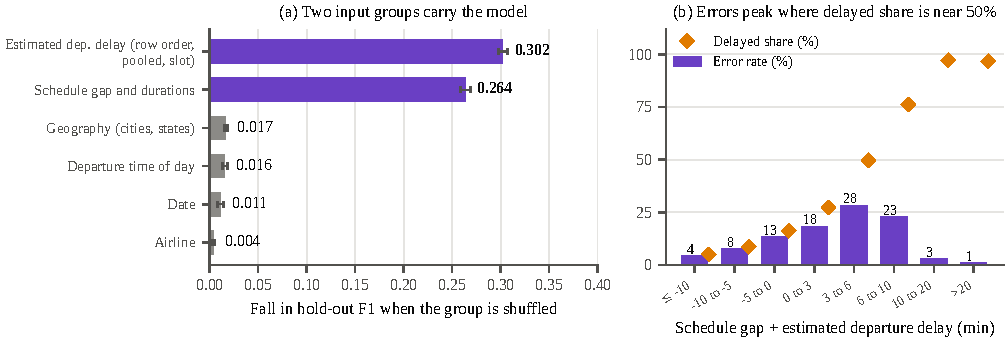
\includegraphics[width=0.92\textwidth]{fig9_errors.pdf}
\caption{Which inputs the Gradient Boosting model relies on and where it errs on the hold-out set. (a) Fall in \Fone{} when a group of input columns is shuffled: the estimated departure delay columns (0.302) and the schedule gap and duration columns (0.264) dominate, and airline matters least (0.004). (b) Error rate (blue) and delayed share (orange) by the sum of the schedule gap and the estimated departure delay: errors peak at 28\% where about half of the flights are delayed and fall to 3\% or less beyond 10 minutes.}\label{fig:errors}
\end{figure*}

\begin{table}[t]
\caption{Effect of the cut-off on out-of-fold precision, recall and \Fone{} for Gradient Boosting (training part). The chosen cut-off is in bold.}\label{tab:cutoff}
\small\centering\setlength{\tabcolsep}{4pt}
\begin{tabular}{@{}c c ccc@{}}
\toprule
Cut-off & Flagged (\%) & Precision & Recall & \Fone{}\\
\midrule
0.25 & 37.1 & 0.789 & 0.892 & 0.837\\
0.30 & 35.2 & 0.817 & 0.877 & 0.846\\
\textbf{0.42} & \textbf{31.8} & \textbf{0.868} & \textbf{0.840} & \textbf{0.853}\\
0.55 & 29.1 & 0.904 & 0.800 & 0.849\\
0.70 & 25.9 & 0.945 & 0.746 & 0.834\\
\bottomrule
\end{tabular}
\end{table}

\subsection{Cut-off and performance}
The model outputs a probability, and the cut-off converts it to a prediction. Figure~\ref{fig:gb} (a) shows the out-of-fold \Fone{} across cut-offs. The curve is flat near its maximum, and the chosen cut-off of 0.42 flags 31.8\% of flights, close to the true delayed share of 32.8\%. On the hold-out, the model reaches precision 0.860, recall 0.847, \Fone{} 0.853, accuracy 0.904 and AUC 0.962. Of 8,527 flights, 2,370 delayed flights were found, 429 were missed and 386 on-time flights were flagged (Figure~\ref{fig:gb} (b)). In-sample \Fone{} is 0.904, 5 points above the cross-validated value, which indicates moderate and expected over-fitting. Errors are concentrated near the decision boundary: the 16\% of hold-out flights with a predicted probability between 0.2 and 0.8 account for 63\% of the 815 errors, whereas flights scored below 0.05 or above 0.95 are misclassified only 1.6\% and 0.7\% of the time. This is consistent with the label depending on a margin of a few minutes (Table~\ref{tab:hidden}, row 4), which no feature fully resolves. Figure~\ref{fig:errors} (b) locates the errors: for the 95\% of hold-out flights with both elapsed and scheduled time recorded, the error rate is 28\% where the sum of the schedule gap and the estimated departure delay is 3 to 6 minutes, where only about half of the flights are delayed, and it falls to 3\% or less beyond 10 minutes and to 4\% below $-10$ minutes. The remaining errors are therefore mostly flights that finished within a few minutes of the point where the label switches on, the margin identified in Table~\ref{tab:hidden}, row 4.

Table~\ref{tab:cutoff} shows the trade-off around the chosen cut-off. \Fone{} weights precision and recall equally, so the optimum is a compromise: lowering the cut-off to 0.25 would find 89\% of delayed flights but only 79\% of the flags would be correct, and raising it to 0.70 would make 95\% of flags correct but miss a quarter of delayed flights. An operator who values catching delays more than avoiding false alarms (for example, to pre-position ground staff) would choose a lower cut-off, and one who acts on each flag at a cost would choose a higher one.



\begin{figure*}[t]\figrule\vspace{1pt}
\centering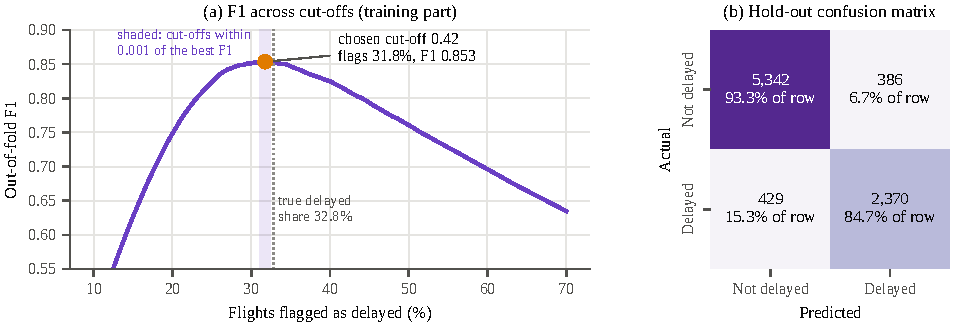
\includegraphics[width=0.92\textwidth]{fig7_gb.pdf}
\caption{Gradient Boosting. (a) Out-of-fold \Fone{} against the share of flights flagged: the curve is flat near its maximum, so the chosen cut-off of 0.42 (31.8\% of flights flagged, \Fone{} 0.853) does not rest on a fragile peak. (b) Hold-out confusion matrix at that cut-off: 84.7\% of delayed flights are found and 93.3\% of on-time flights are correctly left unflagged.}\label{fig:gb}
\end{figure*}

\subsection{Robustness checks}\label{sec:robust}
Two further checks tested whether the result could be improved cheaply. A wider random search of 40 settings (learning rate, tree size, leaf size, regularisation, feature fraction and number of bins) gave three-fold cross-validated \Fone{} between 0.849 and 0.854; its best setting reached a hold-out \Fone{} of 0.849, below the 0.851 of the chosen setting in the same comparison (a separate quick experiment with a simpler feature matrix, so its figures differ slightly from the 0.853 of the main model), so the model is insensitive to hyperparameters. Averaging Gradient Boosting with Random Forest and the Neural Network gave five-fold cross-validated \Fone{} of 0.849 to 0.852, against 0.853 for Gradient Boosting alone, so ensembling offered no reliable gain.

\section{Discussion}
\textbf{Features mattered far more than algorithms.} Row-order features lifted every model by 14 to 18 points on the hold-out (Table~\ref{tab:ladder}), whereas tuning, a wider search and ensembling together moved results by 0.5 points or less. This agrees with the hint in the brief that good features usually matter more than a better classifier. It also explains why seven very different model families end about 6 points apart once the key feature is present, and within 3 points among the six non-linear ones.

\textbf{Significance and limits of the row-order finding.} The row-order features are the most significant result of the study, but their meaning is limited. The file order stands in for the scheduled departure time, which an airline already knows from its timetable, so the features are not a discovery about what causes delays; they make a missing column recoverable. In a deployed system the scheduled departure would be an input, and the useful operational finding is the one in Figure~\ref{fig:signals}: arrival delay is largely the departure delay plus the extra time on the route, and the departure delay should therefore be given to the model.

\textbf{Prediction-time availability.} Several of the strongest inputs (elapsed time, air time, wheels-on time and taxi-in time) are realised during or after a flight, so the scores describe retrospective classification of completed flights, not early forecasting. A forecasting model would be limited to what is known at prediction time, such as scheduled departure, route, airline, weather and current operations.

\textbf{Metric alignment.} Aligning the tuning objective and the cut-off with the metric lifted the same Decision Tree from 0.6044 to 0.6407, a cheap gain that should come first.

\textbf{Why tree ensembles led.} Gradient Boosting and Random Forest handle the threshold-like interaction between schedule gap and estimated departure delay directly, and are insensitive to feature scale and to weakly informative columns. KNN is the weakest non-linear model, plausibly because distances are diluted across many features; the SVM and Neural Network need scaling and sit between the two groups.

\textbf{An apparent ceiling.} In a simulation in which a third of the labelled flights was held out as a pseudo-Unknown set, computing the departure delay from the complete daily flight list raised Gradient Boosting \Fone{} from about 0.85 to about 0.87. This suggests that the remaining gap is due to imperfect recovery of the departure delay and not to model choice, and that about 0.87 is a practical upper bound for this feature design. This is a hypothesis supported by one simulation.

\textbf{Reliability.} The estimates are consistent across three splits and across hold-out and Kaggle (Logistic Regression aside), which is the main evidence that the models generalise to the Unknown file. They remain estimates: each cross-validated score uses cut-offs chosen on its own labels and is slightly optimistic, so the hold-out is the cleaner estimate, and only one random hold-out split was used.

\section{Summary}
Seven classifiers were compared for predicting flight arrival delay from 42,634 labelled flights, evaluated by the \Fone{} of the delayed class and checked on 21,318 unlabelled flights through Kaggle. Gradient Boosting performed best (cross-validated \Fone{} 0.853, hold-out 0.853, Kaggle 0.8471), followed by Random Forest (0.8396), SVM (0.8391), Neural Network (0.8362), Decision Tree (0.8275), KNN (0.8168) and Logistic Regression (0.7730). Four findings stand out.
\begin{enumerate}
\item Feature engineering was worth 17 to 19 points on Kaggle, whereas tuning, a wider search and ensembling together were worth 0.5 points or less.
\item The label follows the sum of two signals, the schedule gap and the departure delay: each alone has an AUC of about 0.73 and together they reach 0.903.
\item Tuning for the competition metric, with the cut-off chosen on out-of-fold predictions, added 3.6 points over tuning for accuracy.
\item Cross-validated, hold-out and Kaggle estimates agree within one point for six of the seven models (1.6 points for Logistic Regression).
\end{enumerate}

\section{Conclusion and Future Work}\label{sec:conclusion}
I conclude that Gradient Boosting on features that recover the departure delay is the best choice among the models tested, and that for this dataset the choice of features matters more than the choice of classifier. A caveat applies. The key feature depends on the way the two files were assembled, with rows sorted by scheduled departure time, and a deployed system would instead read the scheduled departure from the airline timetable. The reported scores therefore describe this dataset, and I would not expect the order-based features to transfer to data without that ordering.

In future work, I plan to treat each day's ordered flight list as a sequence and train a transformer~\cite{attention} to learn the ordering structure directly, instead of hand-building the suffix-minimum and pooling features. I would also compare tabular transformers~\cite{fttransformer} with Gradient Boosting, add real timetable, weather and airport-congestion data, use nested cross-validation to remove the small optimism from tuning, and test the models on a second year of data to measure how well they transfer.

\addcontentsline{toc}{section}{References}
\begin{thebibliography}{9}\footnotesize\setlength{\itemsep}{0pt}
\bibitem{sklearn} Pedregosa, F. et al. (2011). Scikit-learn: Machine learning in Python. \emph{Journal of Machine Learning Research}, 12, 2825--2830.
\bibitem{cart} Breiman, L., Friedman, J., Olshen, R. and Stone, C. (1984). \emph{Classification and Regression Trees}. Wadsworth.
\bibitem{knn} Cover, T. and Hart, P. (1967). Nearest neighbor pattern classification. \emph{IEEE Transactions on Information Theory}, 13(1), 21--27.
\bibitem{rf} Breiman, L. (2001). Random forests. \emph{Machine Learning}, 45(1), 5--32.
\bibitem{svm} Cortes, C. and Vapnik, V. (1995). Support-vector networks. \emph{Machine Learning}, 20(3), 273--297.
\bibitem{mlp} Rumelhart, D., Hinton, G. and Williams, R. (1986). Learning representations by back-propagating errors. \emph{Nature}, 323, 533--536.
\bibitem{gb} Friedman, J. H. (2001). Greedy function approximation: a gradient boosting machine. \emph{Annals of Statistics}, 29(5), 1189--1232.
\bibitem{attention} Vaswani, A. et al. (2017). Attention is all you need. \emph{NeurIPS}, 30.
\bibitem{fttransformer} Gorishniy, Y., Rubachev, I., Khrulkov, V. and Babenko, A. (2021). Revisiting deep learning models for tabular data. \emph{NeurIPS}, 34.
\end{thebibliography}

\clearpage
\appendix
\section*{Appendix A. Python code}\addcontentsline{toc}{section}{Appendix A. Python code}
\small The code below is the single submitted notebook \code{flight\_delay\_models.ipynb}, which contains the shared preprocessing once (A.1, A.2) and then the tuning, cut-off and hold-out cells of all seven models (A.3--A.9). The last cells (A.10) write a Kaggle file for every model: the six other models in the folder \code{other\_models/}, which are the files behind the final-version scores in Table~\ref{tab:kaggle}, and finally the file of the selected model, Gradient Boosting, \code{gb\_predictions.csv}. Cell numbers refer to the position of the cell in the notebook; the markdown cells that explain each step are omitted here. The 90/10 and 100/0 columns of Table~\ref{tab:results} come from the same code with only the split line in A.1 changed (\code{test\_size=0.10}, and \code{X\_train, y\_train = X\_all, y\_all}).

\subsection*{A.1 Shared preprocessing, feature engineering and 80/20 split (cells 1--13)}
\begin{lstlisting}[style=code]
# ===== notebook cell 1 =====
import os, glob, time, warnings
import numpy as np, pandas as pd
import matplotlib.pyplot as plt

from sklearn.base import BaseEstimator, TransformerMixin, clone
from sklearn.linear_model import LinearRegression
from sklearn.compose import ColumnTransformer
from sklearn.pipeline import Pipeline
from sklearn.preprocessing import OneHotEncoder, TargetEncoder, StandardScaler
from sklearn.model_selection import train_test_split, StratifiedKFold, RandomizedSearchCV, cross_val_predict
from sklearn.dummy import DummyClassifier
from sklearn.tree import DecisionTreeClassifier, export_text
from sklearn.neighbors import KNeighborsClassifier
from sklearn.ensemble import RandomForestClassifier, HistGradientBoostingClassifier
from sklearn.svm import SVC
from sklearn.neural_network import MLPClassifier
from sklearn.linear_model import LogisticRegression
from sklearn.metrics import (accuracy_score, precision_score, recall_score, f1_score, roc_auc_score,
                             ConfusionMatrixDisplay, confusion_matrix)

warnings.filterwarnings("ignore")
pd.set_option("display.width", 160); pd.set_option("display.max_columns", 40)

# ---------------- configuration ----------------
DATA_DIR     = "."                       # folder holding the three CSV files
OUTPUT_FILE  = "gb_predictions.csv"  # the Kaggle file (Gradient Boosting, written in section 7)
RANDOM_STATE = 42
TARGET       = "Arrival_Delay"

def find(pattern):
    hits = sorted(glob.glob(os.path.join(DATA_DIR, pattern)))
    return hits[0] if hits else None

FLIGHT_PATH, UNKNOWN_PATH, SAMPLE_PATH = find("*Flight*Dataset*.csv"), find("*Unknown*Dataset*.csv"), find("*Submission*Sample*.csv")
print("flight :", FLIGHT_PATH); print("unknown:", UNKNOWN_PATH); print("sample :", SAMPLE_PATH)
missing_files = [n for n, p in [("flight", FLIGHT_PATH), ("unknown", UNKNOWN_PATH), ("sample", SAMPLE_PATH)] if p is None]
assert not missing_files, f"Could not find the {missing_files} file(s) in DATA_DIR={DATA_DIR!r}. Put all three CSVs next to this notebook."
# ===== notebook cell 3 =====
flight = pd.read_csv(FLIGHT_PATH)
raw_date = flight["DATE"].copy()
print("shape:", flight.shape)
display(flight.head())

bal = flight[TARGET].value_counts().rename("rows").to_frame(); bal["share"] = (bal.rows / len(flight)).round(4)
print("\nClass balance:"); display(bal)
print("Majority-class baseline accuracy:", round(bal.share.max(), 4))

miss = flight.isna().sum(); miss = miss[miss > 0].to_frame("missing"); miss["share"] = (miss.missing / len(flight)).round(3)
print("\nMissing values in the labelled file:"); display(miss)

unk_raw = pd.read_csv(UNKNOWN_PATH)
cmp = pd.DataFrame({"labelled": flight.drop(columns=TARGET).isna().mean(), "unknown": unk_raw.isna().mean()})
print("\nShare of values missing: labelled file vs Unknown file (the Unknown file has extra gaps, handled below)")
display(cmp[(cmp > 0).any(axis=1)].round(3))
# ===== notebook cell 5 =====
def fill_dates_by_order(s):
    '''Fill missing DATE from the nearest known neighbour. Only valid if rows are in date order,
    so the ordering is checked first. Returns (dates, was_sorted).'''
    d = pd.to_datetime(s, errors="coerce")
    if d.dropna().is_monotonic_increasing:
        return d.ffill().bfill(), True
    return d, False

class FlightFeatures(BaseEstimator, TransformerMixin):
    '''Fills missing values from other columns and route statistics, then builds the engineered features.
    Lookup tables and small regressions are learned from the data passed to fit (so cross-validation stays honest).'''
    @staticmethod
    def _clock(s):                       # hhmm -> minutes since midnight (NaN stays NaN; 2400 -> 0)
        s = s % 2400
        return s // 100 * 60 + s % 100

    def fit(self, X, y=None):
        X = X.reset_index(drop=True)
        dep_min = self._clock(X.DEPARTURE_TIME)
        est = dep_min + X.ELAPSED_TIME - X.TAXI_IN
        shift = (((self._clock(X.WHEELS_ON) - est + 720) % 1440) - 720); shift = (shift / 60).round() * 60
        T = X.assign(_shift=shift)
        self.sched_city_  = X.groupby(["O_CITY", "D_CITY"])["SCHEDULED_TIME"].median()
        self.sched_state_ = X.groupby(["O_STATE", "D_STATE"])["SCHEDULED_TIME"].median()
        self.dist_city_   = X.groupby(["O_CITY", "D_CITY"])["DISTANCE"].median()
        self.dist_state_  = X.groupby(["O_STATE", "D_STATE"])["DISTANCE"].median()
        self.elap_city_   = X.groupby(["O_CITY", "D_CITY"])["ELAPSED_TIME"].median()
        self.elap_state_  = X.groupby(["O_STATE", "D_STATE"])["ELAPSED_TIME"].median()
        self.tz_state_    = T.groupby(["O_STATE", "D_STATE"])["_shift"].median()
        self.med_ = X[["SCHEDULED_TIME", "DISTANCE", "ELAPSED_TIME", "AIR_TIME"]].median()
        ok = X.SCHEDULED_TIME.notna() & X.ELAPSED_TIME.notna()
        self.lr_sched_ = LinearRegression().fit(X.loc[ok, ["ELAPSED_TIME"]], X.loc[ok, "SCHEDULED_TIME"])
        self.lr_elap_  = LinearRegression().fit(X.loc[ok, ["SCHEDULED_TIME"]], X.loc[ok, "ELAPSED_TIME"])
        ok = X.DISTANCE.notna() & X.AIR_TIME.notna()
        self.lr_dist_  = LinearRegression().fit(X.loc[ok, ["AIR_TIME"]], X.loc[ok, "DISTANCE"])
        # AIR_TIME from elapsed, taxi-in, distance and scheduled time (fitted on the other columns after they are completed)
        c = self._complete(X); ok = X.AIR_TIME.notna()
        self.lr_air_ = LinearRegression().fit(self._air_inputs(X, c)[ok], X.AIR_TIME[ok])
        return self

    def _lookup(self, X, table, a, b):
        return pd.Series(table.reindex(pd.MultiIndex.from_frame(X[[a, b]])).values, index=X.index)

    def _fill(self, X, col, city, state, lr, xcol):
        v = X[col].fillna(self._lookup(X, city, "O_CITY", "D_CITY")).fillna(self._lookup(X, state, "O_STATE", "D_STATE"))
        r = pd.Series(np.nan, index=X.index); okx = X[xcol].notna()
        if okx.any(): r[okx] = lr.predict(X.loc[okx, [xcol]])
        return v.fillna(r).fillna(self.med_[col])

    def _complete(self, X):
        '''Schedule, distance and elapsed time with every gap filled.'''
        sched = self._fill(X, "SCHEDULED_TIME", self.sched_city_, self.sched_state_, self.lr_sched_, "ELAPSED_TIME")
        dist  = self._fill(X, "DISTANCE", self.dist_city_, self.dist_state_, self.lr_dist_, "AIR_TIME")
        # elapsed time = wheels-on - departure + taxi-in, up to a whole number of hours (time zones).
        # Of the candidates, take the one closest to the scheduled time.
        raw = (self._clock(X.WHEELS_ON) - self._clock(X.DEPARTURE_TIME) + X.TAXI_IN) % 1440
        cand = raw.values[:, None] + 60 * np.arange(-4, 5)[None, :]
        gap = np.abs(cand - sched.values[:, None]); gap = np.where(np.isnan(gap), np.inf, gap)
        derived = pd.Series(cand[np.arange(len(X)), gap.argmin(axis=1)], index=X.index).where(raw.notna())
        elapsed = X.ELAPSED_TIME.fillna(derived)
        elapsed = elapsed.fillna(self._lookup(X, self.elap_city_, "O_CITY", "D_CITY")).fillna(self._lookup(X, self.elap_state_, "O_STATE", "D_STATE"))
        elapsed = elapsed.fillna(pd.Series(self.lr_elap_.predict(sched.to_frame("SCHEDULED_TIME")), index=X.index))
        return dict(sched=sched, dist=dist, elapsed=elapsed)

    @staticmethod
    def _air_inputs(X, c):
        return pd.DataFrame({"el": c["elapsed"], "ti": X.TAXI_IN, "di": c["dist"], "sc": c["sched"]})

    def transform(self, X):
        X = X.reset_index(drop=True).copy(); o = pd.DataFrame(index=X.index)
        c = self._complete(X); sched, dist, elapsed = c["sched"], c["dist"], c["elapsed"]
        air = X.AIR_TIME.copy(); miss = air.isna()
        if miss.any(): air[miss] = self.lr_air_.predict(self._air_inputs(X, c)[miss])
        dep_min = self._clock(X.DEPARTURE_TIME)
        tz = self._lookup(X, self.tz_state_, "O_STATE", "D_STATE").fillna(0)
        est = (dep_min + elapsed - X.TAXI_IN + tz) % 1440
        arr_min = self._clock(X.WHEELS_ON).where(X.WHEELS_ON.notna(), est)
        d = pd.to_datetime(X["DATE"], errors="coerce")
        # raw columns (completed)
        o["DEPARTURE_MIN"] = dep_min; o["SCHEDULED_TIME"] = sched; o["ELAPSED_TIME"] = elapsed
        o["AIR_TIME"] = air; o["DISTANCE"] = dist; o["ARRIVAL_MIN"] = arr_min; o["TAXI_IN"] = X.TAXI_IN
        # schedule gap
        o["DIFF"] = elapsed - sched; o["DIFF_RATIO"] = elapsed / sched
        # time of day
        o["DEP_HOUR"] = dep_min // 60; o["DEP_PRE_DAWN"] = (o.DEP_HOUR < 4).astype(int)
        o["DEP_SIN"] = np.sin(2 * np.pi * dep_min / 1440); o["DEP_COS"] = np.cos(2 * np.pi * dep_min / 1440)
        o["ARR_HOUR"] = arr_min // 60; o["TZ_SHIFT"] = tz
        # taxi / speed
        o["TAXI_OUT"] = elapsed - air - X.TAXI_IN; o["SPEED"] = dist / air
        # calendar
        o["MONTH"] = d.dt.month.fillna(0); o["DOW"] = d.dt.dayofweek.fillna(-1)
        o["DOY"] = d.dt.dayofyear.fillna(0); o["WEEKEND"] = (d.dt.dayofweek >= 5).astype(int)
        # categorical
        o["AIRLINE_NAME"] = X.AIRLINE_NAME
        o["K_DATE"] = d.dt.strftime("%Y-%m-%d").fillna("UNK")
        # geography keys: used for imputation above; only offered to models in the ablation test (row G)
        o["K_O_CITY"] = X.O_CITY.fillna("UNK"); o["K_D_CITY"] = X.D_CITY
        o["K_O_STATE"] = X.O_STATE; o["K_D_STATE"] = X.D_STATE
        return o

RAW  = ["DEPARTURE_MIN", "SCHEDULED_TIME", "ELAPSED_TIME", "AIR_TIME", "DISTANCE", "ARRIVAL_MIN", "TAXI_IN"]
GAP  = ["DIFF", "DIFF_RATIO"]
TOD  = ["DEP_HOUR", "DEP_PRE_DAWN", "DEP_SIN", "DEP_COS", "ARR_HOUR", "TZ_SHIFT"]
TAXI = ["TAXI_OUT", "SPEED"]
CAL  = ["MONTH", "DOW", "DOY", "WEEKEND"]

def make_pre_custom(num, te, scale):
    tr = [("num", StandardScaler() if scale else "passthrough", num),
          ("air", OneHotEncoder(handle_unknown="ignore"), ["AIRLINE_NAME"])]
    if te:
        enc = TargetEncoder(target_type="binary", cv=5, smooth="auto", random_state=RANDOM_STATE)
        tr.append(("te", Pipeline([("enc", enc)] + ([("sc", StandardScaler())] if scale else [])), te))
    return ColumnTransformer(tr)

# three named feature sets (the distance-based models may choose among them)
FEATURE_SETS = {"full":         dict(num=RAW + GAP + TOD + TAXI + CAL, te=["K_DATE"]),
                "compact":      dict(num=RAW + GAP,                    te=[]),
                "compact+date": dict(num=RAW + GAP,                    te=["K_DATE"])}
def make_pre(name, scale): return make_pre_custom(FEATURE_SETS[name]["num"], FEATURE_SETS[name]["te"], scale)
def make_pipe(clf, fset="full", scale=False):
    return Pipeline([("feat", FlightFeatures()), ("pre", make_pre(fset, scale)), ("clf", clf)])

# fill DATE once (a deterministic cleaning step that never touches the target)
flight["DATE"], date_sorted = fill_dates_by_order(flight["DATE"])
print("File is date-sorted:", date_sorted, "| dates still missing:", int(flight.DATE.isna().sum()))
# ===== notebook cell 7 =====
def _clock(s):
    s = s % 2400
    return s // 100 * 60 + s % 100

def order_features(df):
    """Row-order features for one file (rows in original file order, DATE filled). Uses departure times and order only."""
    d = pd.to_datetime(df["DATE"], errors="coerce").values
    dep = _clock(df["DEPARTURE_TIME"]).astype(float).values
    out = {k: np.full(len(df), np.nan) for k in ["SUFMIN", "PREV", "NEXT", "NEXT5", "PREV5", "NEXT10Q", "FRAC", "DEPU"]}
    for day in pd.unique(d):
        idx = np.where(d == day)[0]; v = dep[idx].copy(); m = len(idx)
        frac = np.arange(m) / max(m - 1, 1)
        v[(v < 360) & (frac > 0.5)] += 1440          # departed after midnight although scheduled late in the day
        s = pd.Series(v)
        out["SUFMIN"][idx] = np.minimum.accumulate(v[::-1])[::-1]
        out["PREV"][idx] = s.shift(1).values; out["NEXT"][idx] = s.shift(-1).values
        out["NEXT5"][idx] = s[::-1].shift(1).rolling(5, min_periods=1).median()[::-1].values
        out["PREV5"][idx] = s.shift(1).rolling(5, min_periods=1).median().values
        out["NEXT10Q"][idx] = s[::-1].rolling(10, min_periods=1).quantile(0.2)[::-1].values
        out["FRAC"][idx] = frac; out["DEPU"][idx] = v
    v = out["DEPU"]
    o = pd.DataFrame({"DEP_DELAY_EST": v - out["SUFMIN"], "ROW_FRAC": out["FRAC"]}, index=df.index)
    for k, name in [("PREV", "D_PREV_DEP"), ("NEXT", "D_NEXT_DEP"), ("NEXT5", "D_NEXT5_MED"), ("PREV5", "D_PREV5_MED"), ("NEXT10Q", "D_NEXT10_Q20")]:
        o[name] = v - out[k]
    return o.fillna(0.0)                              # first/last flight of a day has no neighbour on one side

ORDER_COLS = ["DEP_DELAY_EST", "ROW_FRAC", "D_PREV_DEP", "D_NEXT_DEP", "D_NEXT5_MED", "D_PREV5_MED", "D_NEXT10_Q20"]

# labelled file: two random halves (same density as the Unknown file), features computed within each half, original order kept
half = np.random.default_rng(RANDOM_STATE).random(len(flight)) < 0.5
for mask in (half, ~half):
    of = order_features(flight.loc[mask])
    for c in ORDER_COLS: flight.loc[mask, c] = of[c].values

# Unknown file: features computed within the file, in its own order
unk_tmp = unk_raw.copy(); unk_tmp["DATE"], _ = fill_dates_by_order(unk_tmp["DATE"])
of = order_features(unk_tmp)
for c in ORDER_COLS: unk_raw[c] = of[c].values

from sklearn.metrics import roc_auc_score
print("Flights per day - labelled halves: %.0f / %.0f, Unknown: %.0f" % (
      flight[half].groupby("DATE").size().median(), flight[~half].groupby("DATE").size().median(), unk_tmp.groupby("DATE").size().median()))
tot = flight["DEP_DELAY_EST"] + (flight["ELAPSED_TIME"] - flight["SCHEDULED_TIME"]).fillna(0)
print("How well each signal alone separates delayed from on-time flights (AUC, 0.5 = useless, 1 = perfect):")
print("  schedule gap DIFF            %.3f" % roc_auc_score(flight[TARGET], (flight["ELAPSED_TIME"] - flight["SCHEDULED_TIME"]).fillna(0)))
print("  estimated departure delay    %.3f" % roc_auc_score(flight[TARGET], flight["DEP_DELAY_EST"]))
print("  both added together          %.3f" % roc_auc_score(flight[TARGET], tot))
display(flight[["DATE", "DEPARTURE_TIME"] + ORDER_COLS + [TARGET]].head(12))

# ---- plug the new columns into the modelling pipeline ----
RAW_COLS = [c for c in pd.read_csv(FLIGHT_PATH, nrows=1).columns if c != TARGET]
class WithOrder(BaseEstimator, TransformerMixin):
    """FlightFeatures on the original columns, plus the row-order columns and their sum with the schedule gap."""
    def fit(self, X, y=None):
        self.ff_ = FlightFeatures().fit(X[RAW_COLS]); return self
    def transform(self, X):
        o = self.ff_.transform(X[RAW_COLS])
        oc = X[ORDER_COLS].reset_index(drop=True)
        o = pd.concat([o, oc], axis=1)
        o["TOTAL_DELAY_EST"] = o["DEP_DELAY_EST"] + o["DIFF"]
        return o

ORDER_NUM = ORDER_COLS + ["TOTAL_DELAY_EST"]
FEATURE_SETS = {"full":         dict(num=RAW + GAP + TOD + TAXI + CAL + ORDER_NUM, te=["K_DATE"]),
                "compact":      dict(num=RAW + GAP + ORDER_NUM,                    te=[]),
                "compact+date": dict(num=RAW + GAP + ORDER_NUM,                    te=["K_DATE"])}
def make_pipe(clf, fset="full", scale=False):
    return Pipeline([("feat", WithOrder()), ("pre", make_pre(fset, scale)), ("clf", clf)])
# ===== notebook cell 9 =====
def _bounds(df):
    """Own-list bounds on each flight's scheduled departure: L = previous on-time flight's departure, U = suffix minimum."""
    d = pd.to_datetime(df["DATE"]).values; dep = _clock(df["DEPARTURE_TIME"]).astype(float).values
    L = np.full(len(df), -1e9); U = np.zeros(len(df)); V = np.zeros(len(df))
    for day in pd.unique(d):
        idx = np.where(d == day)[0]; v = dep[idx].copy(); m = len(v); fr = np.arange(m) / max(m - 1, 1)
        v[(v < 360) & (fr > 0.5)] += 1440
        suf = np.minimum.accumulate(v[::-1])[::-1]; anc = np.where(v <= suf + 0.5, v, -1e9)
        L[idx] = np.maximum.accumulate(np.concatenate([[-1e9], anc[:-1]])); U[idx] = suf; V[idx] = v
    return L, U, V

def pooled_features(parts, window=45, tol=0.5):
    """Pool each flight's bounds with copies of the same flight (route, airline, block time) within +/- window days, in all lists."""
    rows = []
    for k, df in enumerate(parts):
        L, U, V = _bounds(df)
        key = (df["O_CITY"].fillna(df["O_STATE"]).astype(str) + "|" + df["D_CITY"].astype(str) + "|" +
               df["AIRLINE_NAME"].astype(str) + "|" + df["SCHEDULED_TIME"].astype(str)).values
        rows.append(pd.DataFrame({"part": k, "i": np.arange(len(df)), "key": key, "ok": df["SCHEDULED_TIME"].notna().values,
                                  "day": (pd.to_datetime(df["DATE"]) - pd.Timestamp("2015-01-01")).dt.days.values, "L": L, "U": U, "V": V}))
    A = pd.concat(rows, ignore_index=True)
    S = A.U.values.copy(); LB = A.L.values.copy(); N = np.zeros(len(A)); NE = np.zeros(len(A))
    for _, g in A[A.ok].groupby("key"):
        o = np.argsort(g.day.values, kind="stable")
        ii, dd, LL, UU = g.index.values[o], g.day.values[o], g.L.values[o], g.U.values[o]
        for t in range(len(ii)):
            lo = np.searchsorted(dd, dd[t] - window); hi = np.searchsorted(dd, dd[t] + window, side="right")
            cu, cl = UU[lo:hi], LL[lo:hi]
            c = cu[cu >= LL[t] - tol]                      # copies consistent with this flight's own position
            if len(c):
                S[ii[t]] = min(UU[t], c.min()); N[ii[t]] = len(c); NE[ii[t]] = (np.abs(c - c.min()) <= 5).sum()
            cl2 = cl[(cl <= UU[t] + tol) & (cl > -1e8)]
            if len(cl2): LB[ii[t]] = max(LL[t], cl2.max()) if LL[t] > -1e8 else cl2.max()
    A["PDELAY"] = A.V - S; A["PNSUP"] = N; A["PNEAR"] = NE
    A["PDELAY_UB"] = np.where(LB > -1e8, A.V - np.minimum(LB, S), A.PDELAY); A["PWIN"] = np.where(LB > -1e8, S - np.minimum(LB, S), 0)
    cols = ["PDELAY", "PNSUP", "PNEAR", "PDELAY_UB", "PWIN"]
    return [A[A.part == k].sort_values("i")[cols].reset_index(drop=True) for k in range(len(parts))], cols

t0 = time.time()
(p0, p1, pu), POOL_COLS = pooled_features([flight.loc[half], flight.loc[~half], unk_tmp])
for c in POOL_COLS:
    flight.loc[half, c] = p0[c].values; flight.loc[~half, c] = p1[c].values; unk_raw[c] = pu[c].values
print(f"Pooled features computed in {time.time() - t0:.0f}s")
print("AUC alone (0.5 = useless): row-order delay %.3f | pooled delay %.3f | pooled delay + DIFF %.3f" % (
      roc_auc_score(flight[TARGET], flight["DEP_DELAY_EST"]), roc_auc_score(flight[TARGET], flight["PDELAY"]),
      roc_auc_score(flight[TARGET], flight["PDELAY"] + (flight["ELAPSED_TIME"] - flight["SCHEDULED_TIME"]).fillna(0))))

ORDER_COLS = ORDER_COLS + POOL_COLS                    # WithOrder now passes these through as well
class WithOrderPooled(WithOrder):
    def transform(self, X):
        o = super().transform(X); o["PTOTAL_DELAY_EST"] = o["PDELAY"] + o["DIFF"]; return o
ORDER_NUM = ["DEP_DELAY_EST", "ROW_FRAC", "D_PREV_DEP", "D_NEXT_DEP", "D_NEXT5_MED", "D_PREV5_MED", "D_NEXT10_Q20", "TOTAL_DELAY_EST"] + POOL_COLS + ["PTOTAL_DELAY_EST"]
FEATURE_SETS = {"full":         dict(num=RAW + GAP + TOD + TAXI + CAL + ORDER_NUM, te=["K_DATE"]),
                "compact":      dict(num=RAW + GAP + ORDER_NUM,                    te=[]),
                "compact+date": dict(num=RAW + GAP + ORDER_NUM,                    te=["K_DATE"])}
def make_pipe(clf, fset="full", scale=False):
    return Pipeline([("feat", WithOrderPooled()), ("pre", make_pre(fset, scale)), ("clf", clf)])

# keep this version (order + pooled features, no slot columns) for Random Forest, SVM, Neural Network and Logistic Regression
FEATURE_SETS_POOLED, make_pipe_pooled = FEATURE_SETS, make_pipe
# ===== notebook cell 11 =====
class WithSlots(WithOrderPooled):
    """Adds minute-level 5-minute-slot features on top of the order and pooled features."""
    def transform(self, X):
        o = super().transform(X)
        V = _clock(X["DEPARTURE_TIME"]).astype(float).values
        S = V - o["PDELAY"].values                              # pooled schedule estimate (upper bound)
        for k in [5, 10, 15, 30, 60]: o[f"DEP_MOD{k}"] = np.mod(V, k)
        o["TO_NEXT5"] = np.mod(-V, 5); o["FROM_PREV5"] = np.mod(V, 5)
        s_up = np.minimum(np.ceil(V / 5) * 5, np.ceil(S / 5) * 5); s_dn = np.minimum(np.floor(V / 5) * 5, np.floor(S / 5) * 5)
        o["DD_IF_EARLY"] = V - s_up; o["DD_IF_LATE"] = V - s_dn
        o["ARR_IF_EARLY"] = o["DD_IF_EARLY"] + o["DIFF"]; o["ARR_IF_LATE"] = o["DD_IF_LATE"] + o["DIFF"]
        o["S_MOD5"] = np.mod(S, 5)
        return o

SLOT_NUM = ["DEP_MOD5", "DEP_MOD10", "DEP_MOD15", "DEP_MOD30", "DEP_MOD60", "TO_NEXT5", "FROM_PREV5",
            "DD_IF_EARLY", "DD_IF_LATE", "ARR_IF_EARLY", "ARR_IF_LATE", "S_MOD5"]
FEATURE_SETS = {"full":         dict(num=RAW + GAP + TOD + TAXI + CAL + ORDER_NUM + SLOT_NUM, te=["K_DATE"]),
                "compact":      dict(num=RAW + GAP + ORDER_NUM + SLOT_NUM,                    te=[]),
                "compact+date": dict(num=RAW + GAP + ORDER_NUM + SLOT_NUM,                    te=["K_DATE"])}
def make_pipe(clf, fset="full", scale=False):
    return Pipeline([("feat", WithSlots()), ("pre", make_pre(fset, scale)), ("clf", clf)])

# quick evidence for the claim above, on the labelled file
_V = _clock(flight["DEPARTURE_TIME"]).astype(float)
print("Share delayed by DIFF band, for flights whose departure sits in the stream (no later-listed flight left earlier, neighbours within 4 min):")
_d = pd.to_datetime(flight["DATE"])
_nxt = _V.groupby([_d, half]).shift(-1); _prv = _V.groupby([_d, half]).shift(1)
_tight = (flight["DEP_DELAY_EST"] == 0) & (_nxt - _V).between(0, 4) & (_V - _prv).between(0, 4)
_diff = flight["ELAPSED_TIME"] - flight["SCHEDULED_TIME"]
print(flight.loc[_tight, TARGET].groupby(pd.cut(_diff[_tight], [-60, 0, 2, 5, 8, 10, 15, 90])).agg(["size", "mean"]).round(3).to_string())

# keep this version (pooled + slot columns) for Decision Tree, KNN and Gradient Boosting
FEATURE_SETS_SLOTS, make_pipe_slots = FEATURE_SETS, make_pipe
# ===== notebook cell 13 =====
FEATURE_COLS = [c for c in flight.columns if c != TARGET]
X_all, y_all = flight[FEATURE_COLS], flight[TARGET]
X_train, X_test, y_train, y_test = train_test_split(X_all, y_all, test_size=0.20, stratify=y_all, random_state=RANDOM_STATE)
print(f"training : {X_train.shape[0]:>6} rows  ({X_train.shape[0] / len(X_all):.0%}), delayed share {y_train.mean():.3f}")
print(f"hold-out : {X_test.shape[0]:>6} rows  ({X_test.shape[0] / len(X_all):.0%}), delayed share {y_test.mean():.3f}")
\end{lstlisting}
\subsection*{A.2 Shared tools: scorer, cut-off choice and hold-out check (cell 15)}
\begin{lstlisting}[style=code]
# ===== notebook cell 15 =====
RESULTS, MODELS = {}, {}

def use_features(kind):
    """'pooled' = order + pooled features (RF, SVM, NN, LR); 'slots' = pooled + 5-minute-slot columns (DT, KNN, GB)."""
    global FEATURE_SETS, make_pipe, PRE_SCALED
    FEATURE_SETS, make_pipe = (FEATURE_SETS_POOLED, make_pipe_pooled) if kind == "pooled" else (FEATURE_SETS_SLOTS, make_pipe_slots)
    PRE_SCALED = [make_pre(k, True) for k in FEATURE_SETS]       # the three feature sets, standardised

def scores_of(est, X):                    # probability of "delayed" (or the decision score, for models without probabilities)
    return est.predict_proba(X)[:, 1] if hasattr(est, "predict_proba") else est.decision_function(X)

def best_cutoff_f1(est, X, y):            # best F1 over cut-offs that flag 15%-60% of flights as delayed
    s = scores_of(est, X); cuts = np.quantile(s, np.linspace(0.40, 0.85, 19))
    return max(f1_score(y, s >= c) for c in cuts)

def fset_label(ct):                        # readable name of a feature set (for printing)
    names = [t[0] for t in ct.transformers]
    for k, v in FEATURE_SETS.items():
        if v["num"] == ct.transformers[0][2] and bool(v["te"]) == ("te" in names): return k

def choose_cutoff(tree, CV):
    """Out-of-fold scores on the training part -> the F1-maximising cut-off (middle of the near-best plateau)."""
    METHOD = "predict_proba" if hasattr(tree, "predict_proba") else "decision_function"
    oof = cross_val_predict(tree, X_train, y_train, cv=CV, method=METHOD, n_jobs=-1)
    if oof.ndim == 2: oof = oof[:, 1]
    cuts = np.unique(np.quantile(oof, np.linspace(0.30, 0.90, 121)))
    f1_curve = np.array([f1_score(y_train, oof >= c) for c in cuts])
    good = cuts[f1_curve >= f1_curve.max() - 0.001]                 # middle of the near-best plateau, not a single noisy peak
    THRESHOLD = float(np.median(good))
    share = (oof >= THRESHOLD).mean()
    print(f"Chosen cut-off: {THRESHOLD:.4f}  -> flags {share:.1%} of flights as delayed; out-of-fold F1 {f1_score(y_train, oof >= THRESHOLD):.4f}")
    plt.figure(figsize=(6, 3.4))
    plt.plot([(oof >= c).mean() for c in cuts], f1_curve)
    plt.axvline(share, color="C3", ls="--", label="chosen cut-off"); plt.axvline(y_train.mean(), color="grey", ls=":", label="true delayed share")
    plt.xlabel("share of flights flagged as delayed"); plt.ylabel("F1 (out-of-fold, training part)"); plt.legend(); plt.tight_layout(); plt.show()
    return oof, THRESHOLD, share

def row(y, pred, score):
    return dict(accuracy=accuracy_score(y, pred), precision=precision_score(y, pred, zero_division=0), recall=recall_score(y, pred), F1=f1_score(y, pred), AUC=roc_auc_score(y, score))

def holdout_check(name, tree, oof, THRESHOLD):
    """In-sample vs cross-validated vs hold-out F1 at the chosen cut-off, plus the hold-out confusion matrix."""
    dummy = DummyClassifier(strategy="most_frequent").fit(X_train, y_train)
    s, s_train = scores_of(tree, X_test), scores_of(tree, X_train)
    res = pd.DataFrame([dict(accuracy=accuracy_score(y_test, dummy.predict(X_test)), precision=0.0, recall=0.0, F1=0.0, AUC=0.5),
                        row(y_test, tree.predict(X_test), s),
                        row(y_train, (s_train >= THRESHOLD).astype(int), s_train),
                        row(y_train, (oof >= THRESHOLD).astype(int), oof),
                        row(y_test, (s >= THRESHOLD).astype(int), s)],
                       index=["Always predict 'not delayed' (hold-out)", "Model's default rule (hold-out)", "IN-SAMPLE, chosen cut-off", "CROSS-VALIDATED, chosen cut-off", "HOLD-OUT, chosen cut-off"])
    display(res.round(4))
    print(f"In-sample minus hold-out F1: {res.iloc[2].F1 - res.iloc[4].F1:+.4f}   |   cross-validated minus hold-out F1: {res.iloc[3].F1 - res.iloc[4].F1:+.4f}")
    print("What matters is that cross-validated and hold-out agree to within about 1 point: then the skill is real and not memorised.")
    print("Rough size of the sampling error on 8,500 flights: about +/- 1 percentage point. Do not tweak settings to push the hold-out number up.")
    fig, ax = plt.subplots(figsize=(4.8, 4.2))
    ConfusionMatrixDisplay.from_predictions(y_test, (s >= THRESHOLD).astype(int), display_labels=["Not delayed", "Delayed"], cmap="Blues", ax=ax)
    ax.set_title(f"{name} - hold-out confusion matrix"); plt.tight_layout(); plt.show()
    return res

def record(name, search, tree, oof, THRESHOLD, share, res):
    h = lambda p: res[res.index.str.startswith(p)].F1.iloc[0]
    MODELS[name] = dict(tree=tree, threshold=THRESHOLD)
    RESULTS[name] = {"CV F1": h("CROSS-VALIDATED"), "hold-out F1": h("HOLD-OUT"), "in-sample F1": h("IN-SAMPLE"),
                     "cut-off": THRESHOLD, "flagged": share, "search F1": search.best_score_}
\end{lstlisting}
\subsection*{A.3 Decision Tree (cells 19--24)}
\begin{lstlisting}[style=code]
# ===== notebook cell 19 =====
use_features("slots")
CV5 = StratifiedKFold(5, shuffle=True, random_state=RANDOM_STATE)
CUTS = np.round(np.arange(0.10, 0.801, 0.05), 2)
def tree_cutoff_f1(est, X, y):
    p = est.predict_proba(X)[:, 1]
    return max(f1_score(y, p >= t) for t in CUTS)

space = {"clf__max_depth": [4, 6, 8, 10, 12, 16, 20, None], "clf__min_samples_leaf": [10, 20, 30, 50, 75, 100, 150, 200],
         "clf__criterion": ["gini", "entropy"], "clf__ccp_alpha": [0, 5e-5, 1e-4, 2e-4, 5e-4, 1e-3],
         "clf__class_weight": [None, "balanced", {0: 1, 1: 1.5}], "clf__max_leaf_nodes": [None, 30, 60, 120, 250],
         "clf__min_impurity_decrease": [0, 1e-4, 5e-4]}

t0 = time.time()
search = RandomizedSearchCV(make_pipe(DecisionTreeClassifier(random_state=RANDOM_STATE), "full", False), space, n_iter=60, cv=CV5,
                            scoring=tree_cutoff_f1, n_jobs=-1, random_state=RANDOM_STATE)
search.fit(X_train, y_train)
tree = search.best_estimator_
i = search.best_index_
print(f"Done in {time.time() - t0:.0f}s")
print("Best settings:", {k.replace("clf__", ""): v for k, v in search.best_params_.items()})
print(f"Cross-validated F1 (best cut-off) on the training part: {search.best_score_:.4f} (+/- {search.cv_results_['std_test_score'][i]:.4f} between folds)")
print(f"The fitted tree has {tree.named_steps['clf'].get_n_leaves()} leaves and depth {tree.named_steps['clf'].get_depth()}")

cols = ["param_clf__max_depth", "param_clf__min_samples_leaf", "param_clf__max_leaf_nodes", "param_clf__class_weight", "param_clf__criterion", "mean_test_score", "std_test_score"]
top = pd.DataFrame(search.cv_results_)[cols]; top.columns = ["max_depth", "min_leaf", "max_leaves", "class_weight", "criterion", "cv_F1", "std"]
print("\nTop 8 of the 60 settings tried:"); display(top.sort_values("cv_F1", ascending=False).head(8).round(4).reset_index(drop=True))
# ===== notebook cell 21 =====
oof = cross_val_predict(tree, X_train, y_train, cv=CV5, method="predict_proba")[:, 1]
grid = np.round(np.arange(0.10, 0.801, 0.025), 3)
f1_curve = np.array([f1_score(y_train, oof >= t) for t in grid])
# pick the middle of the near-best plateau rather than a single noisy peak
good = grid[f1_curve >= f1_curve.max() - 0.001]
THRESHOLD = float(np.round(np.median(good), 3))
print(f"Chosen cut-off: {THRESHOLD}   (out-of-fold F1 {f1_score(y_train, oof >= THRESHOLD):.4f}; the single best cut-off in the grid was {grid[f1_curve.argmax()]} with {f1_curve.max():.4f})")

plt.figure(figsize=(6, 3.4))
plt.plot(grid, f1_curve, marker="o", ms=3); plt.axvline(0.5, color="grey", ls="--", label="default 0.5")
plt.axvline(THRESHOLD, color="C3", ls="--", label=f"chosen {THRESHOLD}")
plt.xlabel("probability cut-off for 'delayed'"); plt.ylabel("F1 (out-of-fold, training part)"); plt.legend(); plt.tight_layout(); plt.show()
# ===== notebook cell 23 =====
dummy = DummyClassifier(strategy="most_frequent").fit(X_train, y_train)
s = tree.predict_proba(X_test)[:, 1]; s_train = tree.predict_proba(X_train)[:, 1]
def row(y, pred, score):
    return dict(accuracy=accuracy_score(y, pred), precision=precision_score(y, pred, zero_division=0), recall=recall_score(y, pred), F1=f1_score(y, pred), AUC=roc_auc_score(y, score))
res = pd.DataFrame([dict(accuracy=accuracy_score(y_test, dummy.predict(X_test)), precision=0.0, recall=0.0, F1=0.0, AUC=0.5),
                    row(y_train, (s_train >= THRESHOLD).astype(int), s_train),
                    row(y_train, (oof >= THRESHOLD).astype(int), oof),
                    row(y_test, (s >= THRESHOLD).astype(int), s)],
                   index=["Always predict 'not delayed' (hold-out)", f"IN-SAMPLE, cut-off {THRESHOLD}", f"CROSS-VALIDATED, cut-off {THRESHOLD}", f"HOLD-OUT, cut-off {THRESHOLD}"])
display(res.round(4))
gap = res.iloc[1].F1 - res.iloc[3].F1
print(f"In-sample minus hold-out F1: {gap:+.4f}   |   cross-validated minus hold-out F1: {res.iloc[2].F1 - res.iloc[3].F1:+.4f}")
print("A small in-sample gap (a few points) is normal for any tree. What matters is that cross-validated and hold-out agree to within about 1 point, which means the tree's skill is real and not memorised.")
print("Rough size of the sampling error on 8,500 flights: about +/- 1 percentage point. Do not tweak settings to push the hold-out number up.")

fig, ax = plt.subplots(figsize=(4.8, 4.2))
ConfusionMatrixDisplay.from_predictions(y_test, (s >= THRESHOLD).astype(int), display_labels=["Not delayed", "Delayed"], cmap="Blues", ax=ax)
ax.set_title(f"Decision Tree - hold-out confusion matrix (cut-off {THRESHOLD})"); plt.tight_layout(); plt.show()

h = lambda p: res[res.index.str.startswith(p)].F1.iloc[0]
MODELS["Decision Tree"] = dict(tree=tree, threshold=THRESHOLD)
RESULTS["Decision Tree"] = {"CV F1": h("CROSS-VALIDATED"), "hold-out F1": h("HOLD-OUT"), "in-sample F1": h("IN-SAMPLE"),
                            "cut-off": THRESHOLD, "flagged": (oof >= THRESHOLD).mean(), "search F1": search.best_score_}
# ===== notebook cell 24 =====
# what does a shallow version of the tree say? (depth 3, easy to read; the tuned tree itself is far larger)
small = make_pipe(DecisionTreeClassifier(max_depth=3, min_samples_leaf=50, random_state=RANDOM_STATE), "full", False).fit(X_train, y_train)
print(export_text(small.named_steps["clf"], feature_names=list(small.named_steps["pre"].get_feature_names_out()), max_depth=3, show_weights=True))
print("depth-3 tree hold-out accuracy:", round(accuracy_score(y_test, small.predict(X_test)), 4))
\end{lstlisting}
\subsection*{A.4 K-Nearest Neighbours (cells 27--28)}
\begin{lstlisting}[style=code]
# ===== notebook cell 27 =====
use_features("slots")
CV = StratifiedKFold(3, shuffle=True, random_state=RANDOM_STATE)

base = make_pipe(KNeighborsClassifier(), "compact", True)
space = {"pre": PRE_SCALED, "clf__n_neighbors": [5, 11, 21, 31, 51, 75, 101], "clf__weights": ["uniform", "distance"], "clf__p": [1, 2]}
t0 = time.time()
search = RandomizedSearchCV(base, space, n_iter=20, cv=CV, scoring=best_cutoff_f1, n_jobs=-1, random_state=RANDOM_STATE).fit(X_train, y_train)
tree = search.best_estimator_  # (the fitted, tuned model)

print(f"Done in {time.time() - t0:.0f}s")
print("Best settings:", {k.replace("clf__", ""): (fset_label(v) if k == "pre" else v) for k, v in search.best_params_.items()})
print(f"Cross-validated F1 (best cut-off) on the training part: {search.best_score_:.4f} (+/- {search.cv_results_['std_test_score'][search.best_index_]:.4f} between folds)")
r = pd.DataFrame(search.cv_results_)
r["settings"] = [str({k.replace("clf__", ""): (fset_label(v) if k == "pre" else v) for k, v in p.items()}) for p in r.params]
print(f"\nTop 6 of the {len(r)} settings tried:")
print(r.sort_values("mean_test_score", ascending=False)[["mean_test_score", "std_test_score", "settings"]].head(6).round(4).to_string(index=False, max_colwidth=130))
# ===== notebook cell 28 =====
oof, THRESHOLD, share = choose_cutoff(tree, CV)
res = holdout_check("KNN", tree, oof, THRESHOLD)
record("KNN", search, tree, oof, THRESHOLD, share, res)
\end{lstlisting}
\subsection*{A.5 Random Forest (cells 31--32)}
\begin{lstlisting}[style=code]
# ===== notebook cell 31 =====
use_features("pooled")
CV = StratifiedKFold(3, shuffle=True, random_state=RANDOM_STATE)

base = make_pipe(RandomForestClassifier(n_jobs=1, random_state=RANDOM_STATE), "full", False)
space = {"clf__n_estimators": [200, 400], "clf__max_depth": [8, 12, 16, None], "clf__min_samples_leaf": [1, 3, 5, 10, 20],
         "clf__max_features": ["sqrt", 0.3, 0.5], "clf__class_weight": [None, "balanced_subsample"]}
t0 = time.time()
search = RandomizedSearchCV(base, space, n_iter=15, cv=CV, scoring=best_cutoff_f1, n_jobs=-1, random_state=RANDOM_STATE).fit(X_train, y_train)
tree = search.best_estimator_

print(f"Done in {time.time() - t0:.0f}s")
print("Best settings:", {k.replace("clf__", ""): (fset_label(v) if k == "pre" else v) for k, v in search.best_params_.items()})
print(f"Cross-validated F1 (best cut-off) on the training part: {search.best_score_:.4f} (+/- {search.cv_results_['std_test_score'][search.best_index_]:.4f} between folds)")
r = pd.DataFrame(search.cv_results_)
r["settings"] = [str({k.replace("clf__", ""): (fset_label(v) if k == "pre" else v) for k, v in p.items()}) for p in r.params]
print(f"\nTop 6 of the {len(r)} settings tried:")
print(r.sort_values("mean_test_score", ascending=False)[["mean_test_score", "std_test_score", "settings"]].head(6).round(4).to_string(index=False, max_colwidth=130))
# ===== notebook cell 32 =====
oof, THRESHOLD, share = choose_cutoff(tree, CV)
res = holdout_check("Random Forest", tree, oof, THRESHOLD)
record("Random Forest", search, tree, oof, THRESHOLD, share, res)
\end{lstlisting}
\subsection*{A.6 Support Vector Machine (cells 35--36)}
\begin{lstlisting}[style=code]
# ===== notebook cell 35 =====
use_features("pooled")
CV = StratifiedKFold(3, shuffle=True, random_state=RANDOM_STATE)

base = make_pipe(SVC(kernel="rbf", cache_size=1000, random_state=RANDOM_STATE), "compact", True)
space = {"pre": PRE_SCALED, "clf__C": [0.5, 1, 2, 5, 10], "clf__gamma": ["scale", 0.01, 0.03, 0.1], "clf__class_weight": [None, "balanced"]}
X_sub, _, y_sub, _ = train_test_split(X_train, y_train, train_size=8000, stratify=y_train, random_state=RANDOM_STATE)
t0 = time.time()
search = RandomizedSearchCV(base, space, n_iter=12, cv=CV, scoring=best_cutoff_f1, n_jobs=-1, random_state=RANDOM_STATE).fit(X_sub, y_sub)
tree = clone(base).set_params(**search.best_params_).fit(X_train, y_train)   # re-fit the winner on the full training part
print("(tuned on an 8,000-flight subsample, re-fitted on all", len(X_train), "training flights)")

print(f"Done in {time.time() - t0:.0f}s")
print("Best settings:", {k.replace("clf__", ""): (fset_label(v) if k == "pre" else v) for k, v in search.best_params_.items()})
print(f"Cross-validated F1 (best cut-off) on the training part: {search.best_score_:.4f} (+/- {search.cv_results_['std_test_score'][search.best_index_]:.4f} between folds)")
r = pd.DataFrame(search.cv_results_)
r["settings"] = [str({k.replace("clf__", ""): (fset_label(v) if k == "pre" else v) for k, v in p.items()}) for p in r.params]
print(f"\nTop 6 of the {len(r)} settings tried:")
print(r.sort_values("mean_test_score", ascending=False)[["mean_test_score", "std_test_score", "settings"]].head(6).round(4).to_string(index=False, max_colwidth=130))
# ===== notebook cell 36 =====
oof, THRESHOLD, share = choose_cutoff(tree, CV)
res = holdout_check("SVM", tree, oof, THRESHOLD)
record("SVM", search, tree, oof, THRESHOLD, share, res)
\end{lstlisting}
\subsection*{A.7 Neural Network (cells 39--40)}
\begin{lstlisting}[style=code]
# ===== notebook cell 39 =====
use_features("pooled")
CV = StratifiedKFold(3, shuffle=True, random_state=RANDOM_STATE)

base = make_pipe(MLPClassifier(max_iter=300, early_stopping=True, n_iter_no_change=10, random_state=RANDOM_STATE), "full", True)
space = {"clf__hidden_layer_sizes": [(32,), (64,), (64, 32), (128, 64)], "clf__alpha": [1e-5, 1e-4, 1e-3, 1e-2], "clf__learning_rate_init": [1e-3, 3e-3]}
t0 = time.time()
search = RandomizedSearchCV(base, space, n_iter=10, cv=CV, scoring=best_cutoff_f1, n_jobs=-1, random_state=RANDOM_STATE).fit(X_train, y_train)
tree = search.best_estimator_

print(f"Done in {time.time() - t0:.0f}s")
print("Best settings:", {k.replace("clf__", ""): (fset_label(v) if k == "pre" else v) for k, v in search.best_params_.items()})
print(f"Cross-validated F1 (best cut-off) on the training part: {search.best_score_:.4f} (+/- {search.cv_results_['std_test_score'][search.best_index_]:.4f} between folds)")
r = pd.DataFrame(search.cv_results_)
r["settings"] = [str({k.replace("clf__", ""): (fset_label(v) if k == "pre" else v) for k, v in p.items()}) for p in r.params]
print(f"\nTop 6 of the {len(r)} settings tried:")
print(r.sort_values("mean_test_score", ascending=False)[["mean_test_score", "std_test_score", "settings"]].head(6).round(4).to_string(index=False, max_colwidth=130))
# ===== notebook cell 40 =====
oof, THRESHOLD, share = choose_cutoff(tree, CV)
res = holdout_check("Neural Network", tree, oof, THRESHOLD)
record("Neural Network", search, tree, oof, THRESHOLD, share, res)
\end{lstlisting}
\subsection*{A.8 Logistic Regression (cells 43--44)}
\begin{lstlisting}[style=code]
# ===== notebook cell 43 =====
use_features("pooled")
CV = StratifiedKFold(5, shuffle=True, random_state=RANDOM_STATE)

base = make_pipe(LogisticRegression(max_iter=3000), "full", True)
space = {"pre": [make_pre("full", True), make_pre("compact+date", True)], "clf__C": [0.01, 0.03, 0.1, 1, 10, 100], "clf__class_weight": [None, "balanced"]}
t0 = time.time()
search = RandomizedSearchCV(base, space, n_iter=12, cv=CV, scoring=best_cutoff_f1, n_jobs=-1, random_state=RANDOM_STATE).fit(X_train, y_train)
tree = search.best_estimator_

print(f"Done in {time.time() - t0:.0f}s")
print("Best settings:", {k.replace("clf__", ""): (fset_label(v) if k == "pre" else v) for k, v in search.best_params_.items()})
print(f"Cross-validated F1 (best cut-off) on the training part: {search.best_score_:.4f} (+/- {search.cv_results_['std_test_score'][search.best_index_]:.4f} between folds)")
r = pd.DataFrame(search.cv_results_)
r["settings"] = [str({k.replace("clf__", ""): (fset_label(v) if k == "pre" else v) for k, v in p.items()}) for p in r.params]
print(f"\nTop 6 of the {len(r)} settings tried:")
print(r.sort_values("mean_test_score", ascending=False)[["mean_test_score", "std_test_score", "settings"]].head(6).round(4).to_string(index=False, max_colwidth=130))
# ===== notebook cell 44 =====
oof, THRESHOLD, share = choose_cutoff(tree, CV)
res = holdout_check("Logistic Regression", tree, oof, THRESHOLD)
record("Logistic Regression", search, tree, oof, THRESHOLD, share, res)
\end{lstlisting}
\subsection*{A.9 Gradient Boosting (cells 47--48)}
\begin{lstlisting}[style=code]
# ===== notebook cell 47 =====
use_features("slots")
CV = StratifiedKFold(5, shuffle=True, random_state=RANDOM_STATE)

base = make_pipe(HistGradientBoostingClassifier(early_stopping=True, validation_fraction=0.1, n_iter_no_change=50, max_iter=3000, random_state=RANDOM_STATE), "full", False)
space = {"clf__learning_rate": [0.02, 0.03, 0.05, 0.1], "clf__max_leaf_nodes": [15, 31, 63], "clf__min_samples_leaf": [20, 30, 50, 100],
         "clf__l2_regularization": [0, 1, 10], "clf__class_weight": [None, "balanced"]}
t0 = time.time()
search = RandomizedSearchCV(base, space, n_iter=15, cv=CV, scoring=best_cutoff_f1, n_jobs=-1, random_state=RANDOM_STATE).fit(X_train, y_train)
tree = search.best_estimator_

print(f"Done in {time.time() - t0:.0f}s")
print("Best settings:", {k.replace("clf__", ""): (fset_label(v) if k == "pre" else v) for k, v in search.best_params_.items()})
print(f"Cross-validated F1 (best cut-off) on the training part: {search.best_score_:.4f} (+/- {search.cv_results_['std_test_score'][search.best_index_]:.4f} between folds)")
r = pd.DataFrame(search.cv_results_)
r["settings"] = [str({k.replace("clf__", ""): (fset_label(v) if k == "pre" else v) for k, v in p.items()}) for p in r.params]
print(f"\nTop 6 of the {len(r)} settings tried:")
print(r.sort_values("mean_test_score", ascending=False)[["mean_test_score", "std_test_score", "settings"]].head(6).round(4).to_string(index=False, max_colwidth=130))
# ===== notebook cell 48 =====
oof, THRESHOLD, share = choose_cutoff(tree, CV)
res = holdout_check("Gradient Boosting", tree, oof, THRESHOLD)
record("Gradient Boosting", search, tree, oof, THRESHOLD, share, res)
\end{lstlisting}
\subsection*{A.10 Comparison of the models and the Kaggle files (cells 50, 52, 54)}
\begin{lstlisting}[style=code]
# ===== notebook cell 50 =====
KAGGLE = {"Gradient Boosting": 0.8471, "Random Forest": 0.8396, "SVM": 0.8391, "Neural Network": 0.8362,
          "Decision Tree": 0.8275, "KNN": 0.8168, "Logistic Regression": 0.7730}      # public leaderboard scores, entered by hand
summary = pd.DataFrame(RESULTS).T[["CV F1", "hold-out F1", "in-sample F1", "cut-off", "flagged"]]
summary["Kaggle"] = pd.Series(KAGGLE)
summary = summary.loc[list(KAGGLE)]
display(summary.round(4))
best = summary["hold-out F1"].idxmax()
print(f"Highest cross-validated F1: {summary['CV F1'].idxmax()} | highest hold-out F1: {best} | highest Kaggle score: {summary['Kaggle'].astype(float).idxmax()}")

ax = summary[["CV F1", "hold-out F1", "Kaggle"]].astype(float).plot.barh(figsize=(7, 4), width=0.8)
ax.set_xlim(0.75, 0.87); ax.invert_yaxis(); ax.set_xlabel("F1 of the delayed class"); ax.legend(loc="lower right"); plt.tight_layout(); plt.show()
# ===== notebook cell 52 =====
# --- read and prepare the Unknown file (same columns as the labelled file, no answers) ---
sample = pd.read_csv(SAMPLE_PATH)
X_unk = unk_raw.copy()
missing_cols = [c for c in FEATURE_COLS if c not in X_unk.columns]
assert not missing_cols, f"Unknown dataset is missing columns: {missing_cols}"
X_unk = X_unk[FEATURE_COLS].copy()
X_unk["DATE"], unk_sorted = fill_dates_by_order(X_unk["DATE"])
print(f"Unknown set: {X_unk.shape} | date-sorted: {unk_sorted} | dates still missing: {int(X_unk.DATE.isna().sum())}")
assert len(X_unk) == len(sample), f"Unknown file has {len(X_unk)} rows but the sample has {len(sample)}"

def write_kaggle(name, path):
    """Re-fit the tuned model on ALL labelled flights, score the Unknown flights, apply the model's cut-off, check the format, save."""
    t0 = time.time()
    tree, THRESHOLD = MODELS[name]["tree"], MODELS[name]["threshold"]
    final = clone(tree)
    if "clf__n_jobs" in final.get_params(): final.set_params(clf__n_jobs=-1)
    final.fit(X_all, y_all)
    pred = (scores_of(final, X_unk) >= THRESHOLD).astype(int)
    sub = pd.DataFrame({"row ID": sample.iloc[:, 0].values, "Predicted_Arrival_Delay": pred})
    assert list(sub.columns) == list(sample.columns), f"columns {list(sub.columns)} != {list(sample.columns)}"
    assert len(sub) == len(sample) and (sub.iloc[:, 0].values == sample.iloc[:, 0].values).all()
    assert set(sub["Predicted_Arrival_Delay"].unique()) <= {0, 1} and sub["Predicted_Arrival_Delay"].notna().all()
    sub.to_csv(path, index=False)
    print(f"Saved {path}: {len(sub)} rows, share predicted delayed = {pred.mean():.3f} (labelled data: {y_all.mean():.3f})  [{time.time() - t0:.0f}s]")
    return sub

# the six other models: one file each, in a separate folder
os.makedirs("other_models", exist_ok=True)
for name in ["Decision Tree", "KNN", "Random Forest", "SVM", "Neural Network", "Logistic Regression"]:
    write_kaggle(name, f"other_models/{name.lower().replace(' ', '_')}_kaggle.csv")
# ===== notebook cell 54 =====
sub = write_kaggle("Gradient Boosting", OUTPUT_FILE)
display(sub.head())
\end{lstlisting}
\end{document}
